\documentclass[11pt]{article}
\usepackage[letterpaper,margin=0.82in]{geometry}
\usepackage[T1]{fontenc}
\IfFileExists{lmodern.sty}{\usepackage{lmodern}}{}
\usepackage{microtype}
\usepackage{amsmath,amssymb,amsthm,mathtools,bm}
\usepackage{booktabs,array,longtable}
\usepackage{enumitem}
\usepackage{xcolor}
\usepackage{tikz}
\usetikzlibrary{arrows.meta,positioning,calc,decorations.pathreplacing}
\usepackage[hidelinks]{hyperref}
\usepackage[nameinlink,capitalise]{cleveref}
\usepackage{fancyhdr}
\usepackage{titlesec}
\usepackage{caption}
\usepackage{float}
\allowdisplaybreaks
\setlength{\emergencystretch}{2em}

\hypersetup{
 pdftitle={Microscopic Origins of Multiplicative Null Interactions in Quantum-Geometric-Nesting Superconductors},
 pdfauthor={Nicholas Sledgianowski}
}
\pagestyle{fancy}
\fancyhf{}
\fancyhead[L]{\small Microscopic origins of multiplicative QGN interactions}
\fancyhead[R]{\small Leakage-integrated revision -- July 28, 2026}
\fancyfoot[C]{\thepage}
\setlength{\headheight}{14pt}
\titleformat{\section}{\large\bfseries}{\thesection.}{0.5em}{}
\titleformat{\subsection}{\normalsize\bfseries}{\thesubsection.}{0.5em}{}
\setlist[itemize]{leftmargin=1.45em,itemsep=0.2em,topsep=0.35em}
\setlist[enumerate]{leftmargin=1.7em,itemsep=0.2em,topsep=0.35em}

\newtheorem{theorem}{Theorem}[section]
\newtheorem{proposition}[theorem]{Proposition}
\newtheorem{lemma}[theorem]{Lemma}
\newtheorem{corollary}[theorem]{Corollary}
\theoremstyle{definition}
\newtheorem{definition}[theorem]{Definition}
\theoremstyle{remark}
\newtheorem{remark}[theorem]{Remark}

\newcommand{\Tr}{\operatorname{Tr}}
\newcommand{\rank}{\operatorname{rank}}
\newcommand{\spec}{\operatorname{spec}}
\newcommand{\Span}{\operatorname{span}}
\newcommand{\I}{\mathrm i}
\newcommand{\e}{\mathrm e}
\newcommand{\Id}{\mathbb I}
\newcommand{\cH}{\mathcal H}
\newcommand{\cZ}{\mathcal Z}
\newcommand{\cR}{\mathcal R}
\newcommand{\cP}{\mathcal P}
\newcommand{\cQ}{\mathcal Q}
\newcommand{\cE}{\mathcal E}
\newcommand{\cL}{\mathcal L}
\newcommand{\cC}{\mathcal C}
\newcommand{\ket}[1]{\lvert #1\rangle}
\newcommand{\bra}[1]{\langle #1\rvert}
\newcommand{\abs}[1]{\lvert #1\rvert}
\newcommand{\norm}[1]{\lVert #1\rVert}
\newcommand{\dd}{\mathrm d}

\title{\textbf{Microscopic Origins of Multiplicative Null Interactions\\in Quantum-Geometric-Nesting Superconductors}\\[0.35em]
\large Pauli-selected bond parity, all-filling current routing, and controlled lattice downfolding}
\author{Nicholas Sledgianowski}
\date{Leakage-integrated research revision, July 28, 2026}

\begin{document}
\maketitle

\begin{abstract}
Quantum-geometric nesting (QGN) supplies positive local interactions with exact paired ground states, but an exact two-block parent faces a sharp transport obstruction: under the additive one-body hypotheses proved self-containedly in Appendix~\ref{app:no-go}, a complete Peierls lift cannot produce off-diagonal hopping between inequivalent pair compositions.  The minimal structural escape in the hypothesis space of that theorem is the multiplicative many-body row $K_x=Q_{a,x}B_x$, where $B_x$ transfers electrons between the channels and $Q_{a,x}$ selects odd simultaneous bond parity.  We derive this row from a conventional multiorbital two-electron interaction class.  The central exact identity is the all-filling current router
\[
 C_{s,x}^{2}B_xP_0=4Q_{s,x}B_xP_0,
 \qquad
 C_{a,x}^{2}B_xP_0=4Q_{a,x}B_xP_0,
\]
which converts ordinary current-path interference into the emergent parity projector.  Under the full high-block gap $D\succeq d_*\mathbb I>0$, a four-orbital control sector then produces the exact local Schur complement $-t_B^2B_x^2/d_s+t_B^2(d_s^{-1}-d_a^{-1})K_x^\dagger K_x$ on every seniority-zero filling; a closed-shell Kramers doubling reproduces the same coefficients through weighted order six.

A periodic array gives two distinct lattice theories.  The matched screened family produces the composition-degenerate target at order $\lambda^6$, with connected overlap, residual block coupling, Kramers double excitation, and the first two Peierls derivatives of the remainder bounded by $O(\lambda^8)$ in local norm.  At fixed $\lambda$, its order-four mismatch tolerance is $O(\lambda^2\bar\alpha)$.  The generic unscreened family instead retains the complete linked order-$\lambda^4$ charge-selection operator.  Its product-AGP compression contains the explicit diagonal selector, while its centered action gives simultaneous order-four leakage outside that manifold.  Six verifier programs audit the exact local identities, the weighted lattice scaling, and the periodic/open charge-leakage formulas.
\end{abstract}

\begin{quote}\small
\textbf{Claim hierarchy.}
\begin{enumerate}[leftmargin=1.6em,itemsep=0.12em,topsep=0.2em]
\item The rank-three reduction, sign obstruction, all-filling current router, product-AGP charge projection, and source-restricted Schur formula are exact finite-dimensional identities.
\item The local active--control theorem is exact provided the complete high block satisfies $D\succeq d_*\Id>0$; positivity only on the routed source is not used as a substitute for invertibility of the full Feshbach block.
\item In the screened periodic family, an explicitly defined finite-order local Schrieffer--Wolff unitary gives $\lambda^6\Delta[H_{\rm base}+\bar\alpha\sum_xK_x^\dagger K_x]$ with a quasi-local $O(\lambda^8)$ low-block remainder and $O(\lambda^8)$ residual block coupling.
\item In the unscreened molecular-shell family, the complete order-$\lambda^4$ charge-selection operator accompanies the order-$\lambda^6$ multiplicative term; its product-AGP compression is diagonal, but its off-manifold singular values are generally nonzero.
\item Exact asymptotic screening is a matched parameter submanifold.  At a fixed design value of $\lambda$, a controlled approximate parent permits an order-four mismatch tube of width $O(\lambda^2\bar\alpha)$ and order-six mismatches of width $O(\bar\alpha)$ in local norm.
\item No exact finite-coupling sum of overlapping gadgets, onsite-density-Hubbard-only realization, material parameter extraction, or dynamical zero-frequency Meissner theorem is claimed.  The base two-block QGN parent is an input.
\end{enumerate}
\end{quote}

\section{Introduction}

Perfect quantum-geometric nesting identifies band-geometric conditions under which local interactions can be constructed with exact fermion-bilinear order, including superconducting order and analytically accessible stiffness \cite{Han2024}.  Flat-band superfluid geometry and projected attractive-Hubbard models supply overlapping frameworks: quantum geometry can control the superfluid weight, while a uniform-pairing condition yields exact paired ground states and an emergent pseudospin symmetry \cite{Peotta2015,Tovmasyan2016}.  These results motivate a broader question.  Can the less conventional null interactions required by multiblock QGN superconductors arise from ordinary microscopic electron processes rather than being postulated directly?

The question becomes sharp when the pairing form has two extensive inequivalent singular subbundles.  The exact zero manifold then contains one product antisymmetrized-geminal-power (AGP) state for every allowed pair composition.  Companion work derives the broader block-resolved response law and the additive one-body Peierls obstruction \cite{SledgianowskiMultiBlock,SledgianowskiNoGo}.  For independent evaluation, Appendix~\ref{app:no-go} restates the precise hypotheses and gives the complete short proof needed here: separate one-pair zero states force every one-body null row to preserve the interaction blocks, and complete Peierls transport contributes only a common commutator source removed by the frustration-free least-squares projection.

A local many-body row evades that conclusion.  On bond $x$ define
\begin{equation}
 K_x=Q_{a,x}B_x,
 \label{eq:intro-K}
\end{equation}
where $B_x$ transfers electrons between the two blocks and $Q_{a,x}$ projects onto odd simultaneous endpoint parity.  Because each product AGP is symmetric under the independent block swaps, $K_x$ annihilates the complete zero manifold, while its Peierls derivative can produce a non-diagonal composition response.  The resulting positive-square parent is exact, local, and fully covariant, but its multiplicative form initially appears engineered.

This paper establishes a microscopic origin for \eqref{eq:intro-K}.  The construction combines three familiar mechanisms: Pauli selection of bright and dark parity channels, multiplet-dependent virtual denominators, and orbital-polarization Coulomb energies.  Strong-coupling expansions of Hubbard and charge-transfer models generate exchange, correlated hopping, and cyclic processes beyond second order \cite{MacDonald1988,Aligia2018}; Schrieffer--Wolff theory supplies the corresponding low-energy transformation \cite{Schrieffer1966,Bravyi2011}.

Structurally, the remote control is a mediator-assisted perturbative gadget: ancilla excitations reproduce a more complicated low-energy operator, as in the Hamiltonian-complexity constructions of Kempe--Kitaev--Regev, Oliveira--Terhal, and Jordan--Farhi \cite{Kempe2006,Oliveira2008,Jordan2008}.  The new element here is that the parity router itself is an exact operator identity on the complete broken-pair source space and at every filling; only the energetic elimination and the overlapping lattice array are perturbative.  This exact source-space identity is what permits a volume-uniform fermionic lattice theorem rather than a one-sector gadget analogy.

The main results are:
\begin{enumerate}
\item $K_x^\dagger K_x$ has an exact rank-three seniority-zero representation involving conventional density and pair-motion operators.
\item Passive above-gap elimination obeys a negative-semidefinite sign theorem.  An isolated odd multiplet produces $-\gamma K_x^\dagger K_x$, whereas the positive sign requires a matched $B_x^2$ channel.
\item A four-site electron plaquette built from one-electron hopping, an onsite seniority gap, and intersite density repulsion generates the needed even/odd simultaneous-parity splitting at the perturbatively minimal fourth order for the two-pair tunneling matrix element.
\item An explicit repulsive crossed-shell constant-interaction tensor contains $+\beta B_x^2$ with $\beta>0$, together with a linked monopole charge polynomial.
\item Ordinary orbital-current paths route the full crossed source into even and odd parity sectors for every local charge and every product-AGP filling.
\item A nested four-orbital control sector produces the exact all-filling local Schur complement $-t_B^2B_x^2/d_s+\alpha K_x^\dagger K_x$ under a full high-block gap; a closed-shell Kramers doubling reproduces the same weighted coefficients through degree six.
\item A screened periodic array produces $\sum_xK_x^\dagger K_x$ at order $\lambda^6$ with the first connected overlap corrections delayed to order $\lambda^8$.  The order-four cancellation must be accurate to $O(\lambda^2\bar\alpha)$ at fixed $\lambda$; without that matching, the generic unscreened array retains the complete order-$\lambda^4$ charge-selection operator, whose product-AGP compression contains an explicit diagonal selector and whose centered action generally leaks outside the composition manifold.
\end{enumerate}

\section{Two-block parent and the multiplicative escape}
\label{sec:parent}

\subsection{Active fermions and product-AGP zero manifold}

Let $\Lambda_L=\mathbb Z/L\mathbb Z$.  Each cell contains two blocks $a=1,2$ and spin $\sigma=\uparrow,\downarrow$, with fermions $c_{a,x,\sigma}$.  Define onsite pair operators
\begin{equation}
 d_{a,x}^\dagger=c_{a,x,\uparrow}^\dagger c_{a,x,\downarrow}^\dagger,
 \qquad
 \eta_a^+=\sum_x d_{a,x}^\dagger.
\end{equation}
For $0\le n_a\le L$, the normalized block AGP is
\begin{equation}
 \ket{n_a}_a=\binom{L}{n_a}^{-1/2}(\eta_a^+)^{n_a}\ket0,
\end{equation}
and the two-block product state is $\ket{n_1,n_2}=\ket{n_1}_1\otimes\ket{n_2}_2$.

A convenient exact base parent uses the onsite seniority projectors
\begin{equation}
 q_{a,x}=(n_{a,x,\uparrow}-n_{a,x,\downarrow})^2
\end{equation}
and complete spinful endpoint swaps $W_{a,x}$ on $(x,x+1)$, with
\begin{equation}
 \Pi_{a,x}=\frac{1-W_{a,x}}2.
\end{equation}
Set
\begin{equation}
 H_{\rm base}=\frac{U_0}{2}\sum_{a,x}q_{a,x}
 +\frac12\sum_{a,x}j_a\Pi_{a,x},
 \qquad U_0,j_a>0.
 \label{eq:Hbase}
\end{equation}
The operators $q_{a,x}$ and $\Pi_{a,x}$ are projectors, so the displayed form is positive semidefinite.

\begin{proposition}[Complete base kernel]
\label{prop:base-kernel}
At total particle number $2n$,
\begin{equation}
 \ker H_{\rm base}\big|_{2n}
 =\Span\{\ket{n_1,n_2}:n_1+n_2=n,\ 0\le n_a\le L\}.
 \label{eq:base-kernel}
\end{equation}
Odd-particle sectors have no zero modes.
\end{proposition}

\begin{proof}
The onsite rows force every active orbital to be empty or doubly occupied.  In that hard-core pair space, $\Pi_{a,x}\ket\psi=0$ imposes invariance under every adjacent transposition in block $a$.  Adjacent transpositions generate the full symmetric group $S_L$, whose fixed subspace at pair number $n_a$ is one dimensional and generated by the Dicke/AGP state $\ket{n_a}_a$.  Taking the tensor product over the two blocks proves \eqref{eq:base-kernel}.
\end{proof}

\subsection{Crossed transfer and odd simultaneous parity}

On the oriented bond $x\to x+1$, define
\begin{equation}
\begin{aligned}
 B_x=\sum_\sigma(&c_{1,x+1,\sigma}^\dagger c_{2,x,\sigma}
 +c_{1,x,\sigma}^\dagger c_{2,x+1,\sigma}+\mathrm{H.c.}).
\end{aligned}
\label{eq:Bx}
\end{equation}
Let
\begin{equation}
 W_x=W_{1,x}W_{2,x},
 \qquad
 Q_{s,x}=\frac{1+W_x}{2},
 \qquad
 Q_{a,x}=\frac{1-W_x}{2}.
 \label{eq:Qsa}
\end{equation}
Thus $Q_{a,x}$ is the odd simultaneous-parity projector used throughout the paper.  The verification scripts retain the historical label \texttt{Pi12} for this same operator.
The simultaneous swap exchanges the two crossed paths, hence
\begin{equation}
 [B_x,W_x]=0.
 \label{eq:B-comm-W}
\end{equation}
The multiplicative row and target interaction are
\begin{equation}
 K_x=Q_{a,x}B_x=B_xQ_{a,x},
 \qquad
 H_K=\alpha\sum_xK_x^\dagger K_x,
 \quad \alpha>0.
 \label{eq:K-target}
\end{equation}
Each product AGP is fixed by $W_{1,x}$ and $W_{2,x}$ separately, so $Q_{a,x}\ket{n_1,n_2}=0$ and therefore
\begin{equation}
 K_x\ket{n_1,n_2}=0.
\end{equation}
Thus $H_{\rm base}+H_K$ has at least the complete product-AGP zero manifold.  The companion escape construction proves that it can generate a non-diagonal composition curvature under a complete Peierls twist \cite{SledgianowskiNoGo}.

\begin{figure}[t]
\centering
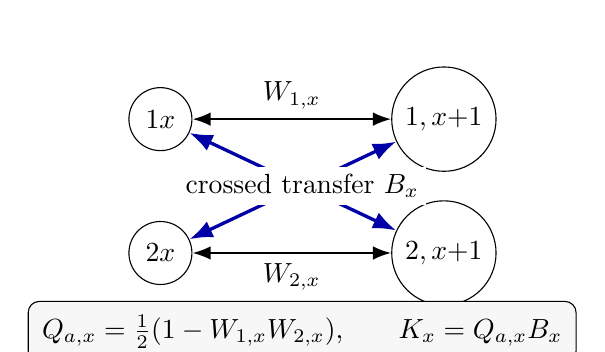
\begin{tikzpicture}[scale=1.0,>=Latex]
 \node[circle,draw,minimum size=8mm] (1L) at (0,0.85) {$1x$};
 \node[circle,draw,minimum size=8mm] (1R) at (3.6,0.85) {$1,x{+}1$};
 \node[circle,draw,minimum size=8mm] (2L) at (0,-0.85) {$2x$};
 \node[circle,draw,minimum size=8mm] (2R) at (3.6,-0.85) {$2,x{+}1$};
 \draw[<->,thick] (1L) -- node[above] {$W_{1,x}$} (1R);
 \draw[<->,thick] (2L) -- node[below] {$W_{2,x}$} (2R);
 \draw[<->,very thick,blue!65!black] (1R) -- (2L);
 \draw[<->,very thick,blue!65!black] (1L) -- (2R);
 \node[fill=white,inner sep=2.5pt,align=center] at (1.8,0) {crossed transfer $B_x$};
 \node[draw,rounded corners,fill=gray!6,align=center,inner sep=5pt] at (1.8,-1.85)
 {$Q_{a,x}=\tfrac12(1-W_{1,x}W_{2,x})$,\qquad $K_x=Q_{a,x}B_x$};
\end{tikzpicture}
\caption{Active two-block bond.  The blue crossed paths form $B_x$.  The simultaneous endpoint swap leaves their sum invariant, while $Q_{a,x}$ selects odd simultaneous parity.}
\label{fig:active-bond}
\end{figure}

\section{Local algebra of the multiplicative interaction}
\label{sec:local-algebra}

\subsection{Full-Fock normal ordering}

For a spinful edge $i\leftrightarrow j$, write
\begin{equation}
 T_{ij}=\sum_\sigma(c_{i\sigma}^\dagger c_{j\sigma}+c_{j\sigma}^\dagger c_{i\sigma}),
\end{equation}
$P_i^\dagger=c_{i\uparrow}^\dagger c_{i\downarrow}^\dagger$, and $S_i^+=c_{i\uparrow}^\dagger c_{i\downarrow}$.  Direct normal ordering yields
\begin{equation}
\boxed{
\begin{aligned}
 T_{ij}^2={}&\sum_\sigma
 (n_{i\sigma}+n_{j\sigma}-2n_{i\sigma}n_{j\sigma})\\
 &+2(P_i^\dagger P_j+P_j^\dagger P_i)
 -2(S_i^+S_j^-+S_i^-S_j^+).
\end{aligned}}
\label{eq:T-square}
\end{equation}
Since the crossed edges are disjoint,
\begin{equation}
 B^2=T_{1L,2R}^2+T_{1R,2L}^2+2T_{1L,2R}T_{1R,2L}.
 \label{eq:B-square-full}
\end{equation}
Thus the ordinary channel $B^\dagger B=B^2$ consists of density terms, singlet pair hopping, transverse spin exchange, and a correlated two-hop term.  The multiplicative interaction conditions those familiar processes on a bond-parity sector.

\subsection{Seniority-zero compression and rank-three form}

On one bond, denote the endpoints by $L,R$.  In seniority zero define $N_{a\ell}=d_{a\ell}^\dagger d_{a\ell}$ and
\begin{equation}
 \mathcal D_\times=\sum_{(i,j)=(1L,2R),(1R,2L)}
 [N_i+N_j-2N_iN_j+d_i^\dagger d_j+d_j^\dagger d_i].
\end{equation}
The block swap becomes
\begin{equation}
 \mathcal W_a=1-N_{aL}-N_{aR}+2N_{aL}N_{aR}
 +d_{aL}^\dagger d_{aR}+d_{aR}^\dagger d_{aL}.
\end{equation}

\begin{proposition}[Exact hard-core reduction]
\label{prop:hardcore-reduction}
Let $P_{\rm sz}$ project the four active orbitals onto seniority zero.  Then
\begin{equation}
 \boxed{P_{\rm sz}B^2P_{\rm sz}=2\mathcal D_\times,}
 \qquad
 \boxed{P_{\rm sz}K^2P_{\rm sz}=(1-\mathcal W_1\mathcal W_2)\mathcal D_\times.}
 \label{eq:hardcore-reduction}
\end{equation}
Moreover, in the occupation basis $\ket{n_{1L}n_{1R}n_{2L}n_{2R}}$, define
\begin{align}
 \ket{u_1}&=\tfrac12(\ket{1000}-\ket{0100}-\ket{0010}+\ket{0001}),\\
 \ket{u_2}&=2^{-1/2}(\ket{1010}-\ket{0101}),\\
 \ket{u_3}&=\tfrac12(\ket{1110}-\ket{1101}-\ket{1011}+\ket{0111}).
\end{align}
Then
\begin{equation}
 \boxed{P_{\rm sz}K^2P_{\rm sz}=4\sum_{m=1}^{3}\ket{u_m}\bra{u_m}.}
 \label{eq:rank-three}
\end{equation}
\end{proposition}

\begin{proof}
Equation \eqref{eq:T-square} compressed to empty/doubly occupied sites gives the density and hard-core pair-hopping terms in $2\mathcal D_\times$; the product of the two disjoint single-electron hops has zero seniority-zero compression.  Since $[B,W_1W_2]=0$, multiplication by $Q_a$ gives the second identity.  Direct action on the sixteen-dimensional hard-core bond basis shows that only the three mutually orthogonal vectors above have nonzero eigenvalue, equal to four.
\end{proof}

The three channels are respectively odd-parity one-pair motion, simultaneous transfer of two pairs between the left and right endpoints, and the particle-hole image of the one-pair process.

\subsection{Why the ordinary \texorpdfstring{$B^2$}{B-squared} channel must be controlled}

On a two-cell bond, the separate one-pair AGPs are
\begin{equation}
 \ket{1,0}=\frac{d_{1L}^\dagger+d_{1R}^\dagger}{\sqrt2}\ket0,
 \qquad
 \ket{0,1}=\frac{d_{2L}^\dagger+d_{2R}^\dagger}{\sqrt2}\ket0.
\end{equation}
Their $B^2$ compression is
\begin{equation}
 \boxed{P_{\cZ_1}B^2P_{\cZ_1}=2
 \begin{pmatrix}1&1\\1&1\end{pmatrix}.}
 \label{eq:B2-compression}
\end{equation}
Hence $B^2$ does not annihilate the full product-AGP zero manifold.  An exact positive-sign completion must cancel its coefficient; an imperfect cancellation is a controlled QGN-breaking perturbation rather than another null interaction.

\section{Sign obstruction and local multiplet completions}
\label{sec:sign-local}

\subsection{Passive second-order sign lemma}

\begin{lemma}[Second-order sign obstruction]
\label{lem:sign}
Let $P$ project onto a low-energy subspace and let $H_Q\succ0$ act on the eliminated subspace $Q=1-P$.  If the perturbation is off diagonal between $P$ and $Q$, then the second-order effective correction is
\begin{equation}
 H_{\rm SW}^{(2)}=-PVQH_Q^{-1}QVP\preceq0.
 \label{eq:SW-sign}
\end{equation}
Consequently, a standalone positive $+\alpha K^\dagger K$ cannot be the sole second-order contribution obtained by eliminating passive above-gap states.
\end{lemma}

\begin{proof}
For every low-energy vector $\ket\psi$,
\begin{equation}
 \bra\psi H_{\rm SW}^{(2)}\ket\psi
 =-\norm{H_Q^{-1/2}QVP\ket\psi}^2\le0.
\end{equation}
\end{proof}

This standard Schrieffer--Wolff sign restriction \cite{Schrieffer1966} explains why the positive multiplicative parent necessarily comes with either a compensating direct channel, a quasienergy denominator of the opposite sign, or a higher-order process.

\subsection{Passive odd-multiplet route}

If only an odd simultaneous-parity multiplet of energy $\Delta_a$ is retained, its coupling matrix is $Q_aB=K$.  The local UV block Hamiltonian
\begin{equation}
 \mathbb H_{\rm pass}=
 \begin{pmatrix}
 H_{\rm base}&tK^\dagger\\
 tK&\Delta_a\Id
 \end{pmatrix}
\end{equation}
has zero-energy Schur complement
\begin{equation}
 H_{\rm pass}=H_{\rm base}-\gamma K^2,
 \qquad \gamma=\frac{t^2}{\Delta_a}.
 \label{eq:passive-eff}
\end{equation}

\begin{lemma}[Sharp odd-sector transfer bound]
\label{lem:sharp-bound}
On the complete local Fock space,
\begin{equation}
 \boxed{K^2\preceq9Q_a.}
 \label{eq:sharp-bound}
\end{equation}
\end{lemma}

\begin{proof}
For the two crossed edges $\mu=1,2$, introduce bonding and antibonding modes $\gamma_{\mu,\pm,\sigma}$ and occupations $N_\pm$.  Then $B=N_+-N_-$.  The simultaneous endpoint swap $W$ exchanges the two crossed edges inside each $\pm$ shell.  Since $N_\pm\in\{0,\ldots,4\}$, the only $\abs B=4$ states are the completely filled $+$ shell and the completely filled $-$ shell.  The edge exchange swaps the two spin-up modes and the two spin-down modes in a filled shell, an even mode permutation, so the induced four-fermion sign is $+1$.  Both states therefore lie in the $W=+1$ sector.  Therefore the spectrum of $B$ on $Q_a\cH$ is contained in $\{-3,-2,-1,0,1,2,3\}$.  Using $[B,Q_a]=0$ gives $K^2=Q_aB^2Q_a\preceq9Q_a$.
\end{proof}

The base exchange estimate
\begin{equation}
 \frac{j_1}{2}\Pi_1+\frac{j_2}{2}\Pi_2\ge\frac{j_{\min}}2Q_a
\end{equation}
and Lemma~\ref{lem:sharp-bound} give the sufficient condition
\begin{equation}
 0\le\gamma<\frac{j_{\min}}{18}
 \quad\Longrightarrow\quad H_{\rm pass}\succeq0
 \label{eq:passive-bound}
\end{equation}
with unchanged zero manifold.  The sign-reversed interaction is therefore already a passive microscopic route to nontrivial composition hopping.

\subsection{Compensated positive route}

Retain even and odd multiplets with
\begin{equation}
 Q_s=1-Q_a,
 \qquad
 H_\Delta=\Delta_sQ_s+\Delta_aQ_a,
 \qquad0<\Delta_s<\Delta_a.
\end{equation}
The UV block
\begin{equation}
 \mathbb H_+=
 \begin{pmatrix}
 H_{\rm base}+\beta B^2&tB\\
 tB&H_\Delta
 \end{pmatrix},
 \qquad \beta=\frac{t^2}{\Delta_s},
 \label{eq:comp-UV}
\end{equation}
has the exact zero-energy Schur complement
\begin{equation}
 \boxed{H_{\rm Schur}(0)=H_{\rm base}+\alpha K^2,}
 \qquad
 \boxed{\alpha=t^2\left(\frac1{\Delta_s}-\frac1{\Delta_a}\right)>0.}
 \label{eq:comp-Schur}
\end{equation}
This isolated block identity is exact, not merely perturbative.  It separates the two microscopic tasks addressed below: generate $\Delta_a>\Delta_s$ without inserting a parity projector, and generate the matched positive $B^2$ coefficient through an ordinary interaction channel.

\section{Electron-only origins of parity and orbital polarization}
\label{sec:electron-only}

\subsection{Pauli selection on a dimer}

For two sites $L,R$, let $\ket{D_L}$ and $\ket{D_R}$ be onsite pairs and let $\ket S$ be the broken-pair spin singlet.  Ordinary hopping with relative phase $\phi$,
\begin{equation}
 T_\phi=t\sum_\sigma(\e^{\I\phi}c_{L\sigma}^\dagger c_{R\sigma}
 +\e^{-\I\phi}c_{R\sigma}^\dagger c_{L\sigma}),
\end{equation}
obeys
\begin{equation}
 QT_\phi P=2t\ket S\bra{P_\phi},
 \qquad
 \ket{P_\phi}=\frac{\e^{\I\phi}\ket{D_L}+\e^{-\I\phi}\ket{D_R}}{\sqrt2}.
 \label{eq:Pauli-selector}
\end{equation}
Only one pair-parity combination is bright; its orthogonal partner is Pauli dark.  At $\phi=\pi/2$ the selected state is the odd pair combination.  The phase on an isolated dimer is gauge dependent, but the same interference is physical in a loop, layer, valley, or molecular-orbital geometry with two distinct paths.

\subsection{Four-site simultaneous-parity plaquette}

Order the active sites as $(1L,1R,2L,2R)$ and consider
\begin{equation}
\boxed{
\begin{aligned}
H_{\rm plaq}={}&
\frac{\Delta_p}{2}\sum_i(n_{i\uparrow}-n_{i\downarrow})^2
+\frac{V_p}{4}(n_{1L}n_{1R}+n_{1R}n_{2L}+n_{2L}n_{2R}+n_{2R}n_{1L})\\
&-t_p\sum_{a=1}^{2}\sum_\sigma(c_{aL\sigma}^\dagger c_{aR\sigma}+\mathrm{H.c.}),
\qquad \Delta_p,V_p>0.
\end{aligned}}
\label{eq:plaquette}
\end{equation}
The first term is an onsite even-occupancy or seniority gap: at fixed charge,
\begin{equation}
 \frac{\Delta_p}{2}(n_{i\uparrow}-n_{i\downarrow})^2
 =\frac{\Delta_p}{2}n_i-\Delta_p n_{i\uparrow}n_{i\downarrow}.
\end{equation}
Thus the plaquette uses ordinary one-electron hopping, an onsite pairing/seniority energy, and intersite density repulsion.

At four electrons and $t_p=0$, the zero doublet is
\begin{equation}
 \ket A=d_{1L}^\dagger d_{2L}^\dagger\ket0,
 \qquad
 \ket B=d_{1R}^\dagger d_{2R}^\dagger\ket0.
\end{equation}
It is separated from adjacent two-pair configurations by $V_p$ and from broken-pair configurations by at least $\Delta_p$.  The simultaneous swap interchanges $\ket A$ and $\ket B$, giving parity eigenstates $\ket s=(\ket A+\ket B)/\sqrt2$ and $\ket a=(\ket A-\ket B)/\sqrt2$.

\begin{proposition}[Electron-generated simultaneous-parity splitting]
\label{prop:plaquette-splitting}
The second-order shifts of $\ket s$ and $\ket a$ are equal.  Their first splitting is fourth order:
\begin{equation}
 E_a-E_s=J_{\rm parity}t_p^4+O(t_p^6),
 \label{eq:parity-splitting}
\end{equation}
where
\begin{equation}
 \boxed{J_{\rm parity}=
 \frac{256(2\Delta_p+3V_p)}
 {V_p(2\Delta_p+V_p)(4\Delta_p+3V_p)^2}>0.}
 \label{eq:Jparity}
\end{equation}
Thus one-electron hopping, the onsite seniority gap, and intersite density repulsion generate an isolated parity doublet with the odd state higher than the even state.
\end{proposition}

\begin{proof}[Proof sketch]
The gauge transformation $c_{aR\sigma}\mapsto-c_{aR\sigma}$ sends $t_p\mapsto-t_p$ while leaving every diagonal term invariant, so the spectrum is even in $t_p$ and all odd orders vanish.  Every second-order virtual walk leaves and returns to the same diagonal pair configuration; the resulting operator on $\Span\{\ket A,\ket B\}$ is proportional to the identity.  A path connecting $\ket A$ to $\ket B$ must move four electrons and therefore first appears at fourth order.  The fourth-order folded term is also proportional to the identity because the second-order operator is scalar on the doublet, so it cancels from $E_a-E_s$.  The connected zero-energy Feshbach path sum gives
\begin{equation}
 h_{AB}^{(4)}=-\frac{128(2\Delta_p+3V_p)}
 {V_p(2\Delta_p+V_p)(4\Delta_p+3V_p)^2}t_p^4.
\end{equation}
Since $E_s-E_a=2h_{AB}^{(4)}+O(t_p^6)$, \eqref{eq:Jparity} follows.  The path organization is given in \cref{app:plaquette}.
\end{proof}

The full $K^2$ operator contains a matrix element transferring two complete pairs.  Since an order-$m$ product of one-electron hoppings can move at most $m$ electrons, that two-pair tunneling/parity-splitting matrix element cannot appear before fourth order.  The plaquette saturates this lower bound.  It does not by itself realize the complete all-filling $K^2$ operator; that role is played by the current router below.

\subsection{The positive \texorpdfstring{$B^2$}{B-squared} channel from repulsive Coulomb interactions}

For each crossed edge, define bonding and antibonding orbitals
\begin{equation}
 \gamma_{\mu,\pm,\sigma}=\frac{c_{i_\mu\sigma}\pm c_{j_\mu\sigma}}{\sqrt2},
 \qquad \mu=1,2,
\end{equation}
and total occupations $N_\pm$.  Then
\begin{equation}
 \boxed{B=N_+-N_-.}
 \label{eq:B-polarization}
\end{equation}
The explicitly repulsive constant-interaction tensor
\begin{equation}
 H_{UV}=\frac{U_c}{2}[N_+(N_+-1)+N_-(N_--1)]+V_cN_+N_-
 \label{eq:Coulomb-shell}
\end{equation}
becomes
\begin{equation}
 \boxed{H_{UV}=A_cN^2-\frac{U_c}{2}N+\beta B^2,}
 \qquad
 A_c=\frac{U_c+V_c}{4},
 \quad
 \beta=\frac{U_c-V_c}{4}.
 \label{eq:Coulomb-decomp}
\end{equation}
For $U_c>V_c>0$, the orbital-polarization coefficient is positive even though all bare density couplings in \eqref{eq:Coulomb-shell} are repulsive.  The construction proves existence within a conventional multiorbital constant-interaction class.  More generally, the corresponding matrix elements are allowed within a general multiorbital Coulomb tensor \cite{Georges2013}; no claim is made that their magnitude is generic in a particular material.

\section{Exact all-filling parity router}
\label{sec:all-filling}

The plaquette demonstrates that parity-resolved excitation energies can emerge from ordinary electrons.  We now construct a canonical control sector whose reduced operator is the full crossed $B$ on every local seniority-zero charge sector.

\subsection{Universal broken-pair source}

On one active bond, let $P_0$ project onto seniority zero and let $P_2$ project onto configurations with exactly two singly occupied active orbitals.

\begin{lemma}[All-filling source identity]
\label{lem:source}
The crossed transfer satisfies
\begin{equation}
 \boxed{P_0BP_0=0,\qquad BP_0=P_2BP_0.}
 \label{eq:source-identity}
\end{equation}
It therefore maps every seniority-zero configuration into the universal source space
\begin{equation}
 \cR=\operatorname{ran}(BP_0)\subset P_2\cH.
\end{equation}
Moreover $[B,W]=0$, so the source retains simultaneous endpoint parity.
\end{lemma}

\begin{proof}
A single one-electron hop cannot map a configuration with only empty and doubly occupied sites back into seniority zero.  Whenever the hop is nonzero, it removes one electron from a pair and places it on an empty crossed endpoint, producing exactly two singly occupied sites.  The simultaneous-swap commutator was established in \eqref{eq:B-comm-W}.
\end{proof}

This statement covers the local zero-, one-, two-, three-, and four-pair sectors and therefore every local component of every global product AGP.

\subsection{Current algebra}

Define the block currents
\begin{equation}
 J_a=\I\sum_\sigma(c_{aL\sigma}^\dagger c_{aR\sigma}-c_{aR\sigma}^\dagger c_{aL\sigma}),
\end{equation}
and the same- and opposite-chirality combinations
\begin{equation}
 C_s=J_1+J_2,
 \qquad
 C_a=J_1-J_2.
 \label{eq:CsCa}
\end{equation}

\begin{lemma}[Exact all-filling parity routing]
\label{lem:routing}
On the low and source spaces,
\begin{align}
 P_0J_a^2P_0&=4\Pi_aP_0,
 &P_0J_1J_2P_0&=0,
 \label{eq:low-current}\\
 (J_1^2-1)BP_0&=0,
 &(J_2^2-1)BP_0&=0,
 \label{eq:range-current1}\\
 (J_1J_2-W)BP_0&=0.
 \label{eq:range-current2}
\end{align}
Consequently,
\begin{equation}
 \boxed{C_s^2BP_0=4Q_sBP_0,\qquad C_a^2BP_0=4Q_aBP_0.}
 \label{eq:routing}
\end{equation}
The operators $C_s^2$ and $C_a^2$ preserve $\cR$.
\end{lemma}

\begin{proof}
The one-block matrices are displayed in \cref{app:current-table}.  On the seniority-zero states $\ket0$, $\ket{D_L}$, $\ket{D_R}$, and $\ket{D_LD_R}$ they give $P_0J_a^2P_0=2(1-W_a)P_0=4\Pi_aP_0$.  Currents from distinct blocks produce incompatible seniority patterns, so $P_0J_1J_2P_0=0$.

Every nonzero term in $BP_0$ leaves each block in an odd local particle sector, $N_a=1$ or $3$.  In either odd sector the table gives $J_a^2=1$.  The current matrices in the one-electron and one-hole sectors have opposite orientation; together with the crossed geometry of $B$, their phases multiply so that applying both currents is exactly the simultaneous endpoint swap.  Thus $(J_1J_2-W)BP_0=0$.  Expanding $(J_1\pm J_2)^2$ proves \eqref{eq:routing}.  Since the right-hand sides lie in $\operatorname{ran}(BP_0)$, the squared currents preserve $\cR$.
\end{proof}

Equation \eqref{eq:routing} is the central microscopic identity: parity projectors arise from interference between ordinary current paths rather than appearing as microscopic vertices.

\subsection{Four-orbital control sector}
\label{sec:control-sector}

The exact local algebra below uses one control orbital flavor.  Microscopically, $r_\mu$ may denote a spin-polarized electron stabilized by exchange or Zeeman splitting, or a spin-suppressed orbital pseudospin.  A strictly electronic time-reversal-invariant realization cannot have a unique odd-electron Kramers ground state.  Appendix~\ref{app:kramers} therefore gives two explicit doubled versions: a sector-wise Kramers doublet with exactly identical Schur coefficients, and a unique even-electron closed shell that reproduces the same weighted degree-four and degree-six coefficients while its first double-excitation correction occurs at degree eight.

Introduce one control electron in orbitals $g,m,s,a$, with $E_{\mu\nu}=r_\mu^\dagger r_\nu$.  A local charging term $U_r(N_r-1)^2$ fixes one control electron.  In that sector take positive control energies $\Delta_m,\Delta_s^{(r)},\Delta_a^{(r)}$ and interactions
\begin{align}
 V_{gm}&=t_BB(E_{mg}+E_{gm}),\nonumber\\
 V_{ms}&=t_sC_s(E_{sm}+E_{ms}),\nonumber\\
 V_{ma}&=t_aC_a(E_{am}+E_{ma}).
 \label{eq:control-vertices}
\end{align}
These are ordinary two-electron scattering vertices.  With the explicit mode-order convention that every active mode precedes every control mode, a spin-conserving active bilinear $h_{ij}=\sum_\sigma v_{ij}c_{i\sigma}^\dagger c_{j\sigma}$ satisfies
\begin{equation}
 h_{ij}E_{\mu\nu}
 =-\sum_\sigma v_{ij}
 c_{i\sigma}^\dagger r_\mu^\dagger c_{j\sigma}r_\nu,
 \label{eq:normal-four-fermion}
\end{equation}
with the Hermitian-conjugate and exchanged-index terms supplying the corresponding antisymmetrized number-conserving interaction tensor.  Reversing the active/control mode convention absorbs the displayed minus sign into the ordered interaction coefficient.  Equivalent gauges may place the current phase either in $v_{ij}$ or in the control transition; Appendix~\ref{app:kramers} uses real transitions with opposite signs on the two Kramers partners.

In the ordered control basis $(g,m,s,a)$,
\begin{equation}
 \mathbb H_{\rm ctrl}=
 \begin{pmatrix}
 0&t_BB&0&0\\
 t_BB&\Delta_m&t_sC_s&t_aC_a\\
 0&t_sC_s&\Delta_s^{(r)}&0\\
 0&t_aC_a&0&\Delta_a^{(r)}
 \end{pmatrix}.
 \label{eq:control-matrix}
\end{equation}
No entry contains $W$, $Q_s$, $Q_a$, or $K$.

\begin{figure}[t]
\centering
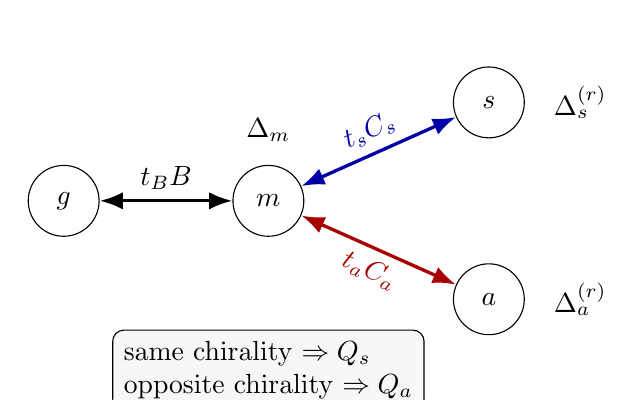
\begin{tikzpicture}[>=Latex]
 \node[circle,draw,minimum size=9mm] (g) at (-2.6,0) {$g$};
 \node[circle,draw,minimum size=9mm] (m) at (0,0) {$m$};
 \node[circle,draw,minimum size=9mm] (s) at (2.8,1.25) {$s$};
 \node[circle,draw,minimum size=9mm] (a) at (2.8,-1.25) {$a$};
 \draw[<->,very thick] (g) -- node[midway,above] {$t_BB$} (m);
 \draw[<->,very thick,blue!65!black] (m) -- node[midway,above,sloped] {$t_sC_s$} (s);
 \draw[<->,very thick,red!65!black] (m) -- node[midway,below,sloped] {$t_aC_a$} (a);
 \node[above=5pt of m] {$\Delta_m$};
 \node[right=7pt of s] {$\Delta_s^{(r)}$};
 \node[right=7pt of a] {$\Delta_a^{(r)}$};
 \node[draw,rounded corners,fill=gray!6,align=left,inner sep=4pt] at (0,-2.15)
 {same chirality $\Rightarrow Q_s$\\opposite chirality $\Rightarrow Q_a$};
\end{tikzpicture}
\caption{Nested active--remote control sector.  The bridge creates the universal source in orbital $m$; two current paths lower its even and odd simultaneous-parity components by different amounts.}
\label{fig:control-chain}
\end{figure}

Eliminating $s$ and $a$ at zero energy gives the full active-space operator
\begin{equation}
 D=\Delta_m-\frac{t_s^2}{\Delta_s^{(r)}}C_s^2
 -\frac{t_a^2}{\Delta_a^{(r)}}C_a^2.
 \label{eq:D-full}
\end{equation}
To define the zero-energy Feshbach map as a full operator, assume
\begin{equation}
 \boxed{D\succeq d_*\Id>0\quad\text{on the complete active Fock space}.}
 \label{eq:D-gap}
\end{equation}
A simple sufficient, though nonoptimal, condition is
\begin{equation}
 \Delta_m>16\left(\frac{t_s^2}{\Delta_s^{(r)}}+\frac{t_a^2}{\Delta_a^{(r)}}\right),
 \label{eq:D-sufficient}
\end{equation}
because $\norm{C_s},\norm{C_a}\le4$.  By Lemma~\ref{lem:routing}, on $\cR$,
\begin{equation}
 D=d_sQ_s+d_aQ_a,
 \label{eq:D-parity}
\end{equation}
where
\begin{equation}
 d_s=\Delta_m-\frac{4t_s^2}{\Delta_s^{(r)}},
 \qquad
 d_a=\Delta_m-\frac{4t_a^2}{\Delta_a^{(r)}}.
 \label{eq:dsa}
\end{equation}
The full-gap assumption implies $d_s,d_a>0$.

\begin{theorem}[Exact all-filling active--remote reduction]
\label{thm:all-filling}
Assume \eqref{eq:D-gap}, and let $F_g(0)$ be the zero-energy Schur complement in the control-ground sector.  On the complete active seniority-zero space,
\begin{equation}
 \boxed{P_0F_g(0)P_0=-\frac{t_B^2}{d_s}P_0B^2P_0+\alpha P_0K^2P_0,}
 \label{eq:all-filling-Schur}
\end{equation}
where
\begin{equation}
 \boxed{\alpha=t_B^2\left(\frac1{d_s}-\frac1{d_a}\right).}
 \label{eq:alpha-local}
\end{equation}
If $t_s^2/\Delta_s^{(r)}>t_a^2/\Delta_a^{(r)}$, then $d_s<d_a$ and $\alpha>0$.
\end{theorem}

\begin{proof}
The full-gap assumption makes
\begin{equation}
 F_g(0)=-t_B^2BD^{-1}B
\end{equation}
well defined.  Since $BP_0\subset\cR$, \eqref{eq:D-parity} gives
\begin{equation}
 D^{-1}BP_0=(d_s^{-1}Q_s+d_a^{-1}Q_a)BP_0.
\end{equation}
Use $Q_s=1-Q_a$, $[B,Q_a]=0$, and $K=Q_aB$.
\end{proof}

For example, $\Delta_m=10$, $\Delta_s^{(r)}=\Delta_a^{(r)}=8$, $t_s=1$, $t_a=1/2$, and $t_B=0.7$ give
\begin{equation}
 d_s=9.5,
 \qquad d_a=9.875,
 \qquad \alpha=1.958694203864\times10^{-3}.
\end{equation}
The full-Fock operator $D$ has minimum eigenvalue $8$ (hence the complete high control block is positive), and the Schur-complement residual is below $2.3\times10^{-17}$.  The value $t_B=0.7$ is an algebraic stress test of the exact source reduction; it is not used below as a quantitatively small finite-coupling compensation benchmark.

The positivity condition $t_s^2/\Delta_s^{(r)}>t_a^2/\Delta_a^{(r)}$ is an open inequality rather than an equality tuning.  No symmetry in the construction forces its sign.  Different orbital overlaps, excitation energies, or screening of the two current channels may favor the same-chirality path, but the present paper treats that dominance as a microscopic parameter condition to be checked in any material extraction, not as a generic prediction.

\section{Coulomb compensation and charge control}
\label{sec:charge}

\subsection{Leading cancellation and its linked charge channel}

Matching the crossed-shell interaction \eqref{eq:Coulomb-decomp} to
\begin{equation}
 \beta=\frac{t_B^2}{d_s}
 \label{eq:beta-match}
\end{equation}
cancels the ordinary $B^2$ term in \eqref{eq:all-filling-Schur} and leaves $+\alpha K^2$ at leading order.  No parity-dependent operator is inserted.  However, in the repulsive constant-interaction shell the same parameters also produce
\begin{equation}
 A_c=\frac{U_c+V_c}{4}\ge\frac{U_c-V_c}{4}=\beta>0,
 \label{eq:A-beta-link}
\end{equation}
so the monopole polynomial is generically of the same weighted order as the direct $B^2$ channel.  The screened and unscreened periodic models must therefore be stated separately.

\subsection{Exact product-AGP projection of the monopole terms}

Let $N_x$ be the total active electron number on the four orbitals of bond $(x,x+1)$ and define
\begin{equation}
 H_{\rm ch}=\sum_x\left(A_cN_x^2-\frac{U_c}{2}N_x\right).
\end{equation}

\begin{proposition}[Charge potential on product AGPs]
\label{prop:charge-potential}
For fixed total pair number $n$, let
\begin{equation}
 \mathcal Z_n=\operatorname{span}\{\ket{n_1,n_2}:n_1+n_2=n\}.
\end{equation}
The compression of $H_{\rm ch}$ to $\mathcal Z_n$ is diagonal:
\begin{equation}
 P_{\mathcal Z_n}H_{\rm ch}P_{\mathcal Z_n}
 =\sum_{n_1+n_2=n}V_{\rm ch}^{(L)}(n_1,n_2)
 \ket{n_1,n_2}\!\bra{n_1,n_2},
\end{equation}
where
\begin{equation}
\boxed{
\begin{aligned}
 V_{\rm ch}^{(L)}(n_1,n_2)={}&A_c\left[
 8n+\frac{8[n_1(n_1-1)+n_2(n_2-1)]}{L-1}
 +\frac{32n_1n_2}{L}\right]-2U_cn,
\end{aligned}}
\label{eq:charge-potential}
\end{equation}
where $n=n_1+n_2$.  Equivalently,
\begin{equation}
 \boxed{V_{\rm ch}^{(L)}(n_1,n_2)=C_L(n)+16A_c\frac{L-2}{L(L-1)}n_1n_2.}
 \label{eq:charge-selector}
\end{equation}
\end{proposition}

\begin{proof}
Within each block, the AGP is the uniform fixed-size subset state.  Hence the one-site pair occupation is $n_a/L$ and the probability that both endpoints of a fixed bond are occupied is $n_a(n_a-1)/[L(L-1)]$.  The two blocks are independent, so cross-block endpoint occupations factor.  Expanding $N_x^2$ and summing the translated bonds yields \eqref{eq:charge-potential}; rearranging at fixed $n$ gives \eqref{eq:charge-selector}.
\end{proof}

\begin{proposition}[Exact periodic charge-leakage action and singular values]
\label{prop:charge-leakage-periodic}
Let
\[
 \mathcal Z_n=\operatorname{span}\{\ket{n_1,n_2}:n_1+n_2=n\},
 \qquad
 R_{{\rm ch},L}^{(n)}=(1-P_{\mathcal Z_n})H_{\rm ch}P_{\mathcal Z_n},
\]
and put $D_L=\sum_x N_x^2$.  For a composition $c=(n_1,n_2)$, write
\[
 \mu_{L;c}=\bra cH_{\rm ch}\ket c.
\]
Then the exact composition-resolved action is
\begin{equation}
 \boxed{
 R_{{\rm ch},L}^{(n)}\ket c
 =\bigl(H_{\rm ch}-\mu_{L;c}\bigr)\ket c
 =A_c\bigl(D_L-\langle D_L\rangle_c\bigr)\ket c.}
 \label{eq:periodic-charge-leakage-action}
\end{equation}
For $L\ge3$, define
\begin{equation}
\boxed{
\begin{aligned}
\sigma_L^2(n_1,n_2)=64\Bigg[&
\frac{n_1(n_1-1)(L-n_1)(L-n_1-1)
+n_2(n_2-1)(L-n_2)(L-n_2-1)}{(L-2)(L-1)^2}\\
&+\frac{2n_1n_2(L-n_1)(L-n_2)(3L-8)}{L^2(L-1)^2}
\Bigg].
\end{aligned}}
\label{eq:periodic-charge-leakage-variance}
\end{equation}
Whenever $\sigma_L(c)>0$, let
\begin{equation}
 \ket{\ell_{L;c}}
 =\frac{(D_L-\langle D_L\rangle_c)\ket c}{\sigma_L(c)}.
 \label{eq:periodic-charge-left-singular-vector}
\end{equation}
The nonzero vectors $\ket{\ell_{L;c}}$ are orthonormal, and
\begin{equation}
 \boxed{
 R_{{\rm ch},L}^{(n)}
 =A_c\!\sum_{\substack{c=(n_1,n_2)\\n_1+n_2=n,\ \sigma_L(c)>0}}
 \sigma_L(c)\ket{\ell_{L;c}}\bra c.}
 \label{eq:periodic-charge-leakage-svd}
\end{equation}
Consequently,
\begin{equation}
 \boxed{
 (R_{{\rm ch},L}^{(n)})^\dagger R_{{\rm ch},L}^{(n)}
 =A_c^2\sum_{n_1+n_2=n}\sigma_L^2(n_1,n_2)
 \ket{n_1,n_2}\!\bra{n_1,n_2},}
 \label{eq:periodic-charge-leakage-gram}
\end{equation}
\begin{equation}
 \boxed{
 \norm{R_{{\rm ch},L}^{(n)}}
 =A_c\max_{n_1+n_2=n}\sigma_L(n_1,n_2),
 \qquad
 \operatorname{rank}R_{{\rm ch},L}^{(n)}
 =\#\{c:\sigma_L(c)>0\}.}
 \label{eq:periodic-charge-leakage-norm}
\end{equation}
For $L=2$, $R_{{\rm ch},2}^{(n)}=0$ in every filling sector.  For $L\ge3$,
$\sigma_L^2(n_1,n_2)=0$ exactly when one block is empty or full and the other
has occupation $0$, $1$, $L-1$, or $L$.
\end{proposition}

\begin{proof}
At fixed total pair number, $\sum_x N_x=4n$ is scalar on the periodic cycle, so
only $A_c D_L$ contributes to the off-manifold block.  Since $D_L$ preserves both
block charges, its centered images from distinct compositions have orthogonal
support.  In a fixed composition sector the product AGP is the uniform
normalized fixed-size subset state, and therefore
\[
 \norm{R_{{\rm ch},L}^{(n)}\ket c}^2
 =A_c^2\operatorname{Var}_c(D_L).
\]
Writing
\[
 E_a=\sum_x X_{a,x}X_{a,x+1},\qquad
 t_{a,x}=X_{a,x}+X_{a,x+1},\qquad
 C=\sum_x t_{1,x}t_{2,x},
\]
gives $D_L=8n+8(E_1+E_2+C)$.  Exact cycle counting yields
\[
 \operatorname{Var}(E_a)=
 \frac{n_a(n_a-1)(L-n_a)(L-n_a-1)}{(L-2)(L-1)^2},
\]
\[
 \operatorname{Var}(C)=
 \frac{2n_1n_2(L-n_1)(L-n_2)(3L-8)}{L^2(L-1)^2}.
\]
Moreover $\mathbb E[C\mid X_1]=4n_1n_2/L$ and likewise after conditioning on
$X_2$, so the mixed covariances vanish.  This proves
\eqref{eq:periodic-charge-leakage-variance}.  Centering proves
\eqref{eq:periodic-charge-leakage-action}; normalization and the orthogonal
block-charge supports prove the SVD, Gram operator, norm, and rank.  The stated
zero set follows term by term from \eqref{eq:periodic-charge-leakage-variance}.
\end{proof}

The nonconstant term in the compressed operator is a positive diagonal selector favoring block-polarized compositions.  It vanishes accidentally at $L=2$.  Proposition~\ref{prop:charge-leakage-periodic} shows that this exact compression does not generally define an invariant product-AGP subspace: the same charge operator has nonvanishing singular values $A_c\sigma_L(c)$, of the same shell order as the selector shift, before the microscopic factor $\lambda^4\Delta$ is restored.  Consequently, a two-cell weighted lattice certificate is blind both to the principal unscreened selector and to its first nontrivial leakage.
For the standard open-path truncation used in finite-system DMRG, endpoint charge makes the linear term non-scalar; the exact compressed selector, leakage SVD, and open zero set are given in \cref{cor:charge-leakage-open}.


\begin{remark}[Order-four isolation gate]
\label{rem:order-four-isolation-gate}
Let $\gamma_L^{(n)}>0$ denote the gap, in dimensionless target units, separating
$\mathcal Z_n$ from its complement for an order-six parent used to isolate the
composition manifold.  The exact periodic leakage-to-gap ratio is
\begin{equation}
 \Xi_L^{(n)}(\lambda)
 =\frac{\lambda^4\norm{R_{{\rm ch},L}^{(n)}}}
 {\lambda^6\gamma_L^{(n)}}
 =\frac{A_c\max_{n_1+n_2=n}\sigma_L(n_1,n_2)}
 {\lambda^2\gamma_L^{(n)}}.
 \label{eq:unscreened-leakage-ratio}
\end{equation}
Thus a nonzero order-four leakage channel is not made small relative to an
order-six isolation gap by taking $\lambda\to0$; an autonomous composition
Hamiltonian requires order-four or stronger protection, or an exact cancellation
of the centered charge action.
\end{remark}

\subsection{Feedback of the direct \texorpdfstring{$B^2$}{B-squared} channel}

If the direct Coulomb term also acts in the high control sector, write $D_\beta=D+\beta B^2$.  The exact compensated operator becomes
\begin{equation}
 P_0[\beta B^2-t_B^2BD_\beta^{-1}B]P_0.
\end{equation}

\begin{proposition}[Resolvent-feedback bound]
\label{prop:feedback}
Assume $D\succeq d_*\Id$ and $\eta=\norm{\beta B^2}<d_*$.  Then
\begin{equation}
\boxed{
\norm{P_0[\beta B^2-t_B^2BD_\beta^{-1}B-\alpha K^2]P_0}
\le\frac{t_B^2\norm{B}^2\eta}{d_*(d_*-\eta)}.
}
\label{eq:feedback-bound}
\end{equation}
Since $\norm{B}=4$ and $\beta=O(t_B^2/d_s)$, the feedback is $O(t_B^4/d_*^3)$.
\end{proposition}

\begin{proof}
Use the resolvent identity
\begin{equation}
 D_\beta^{-1}-D^{-1}=-D^{-1}\beta B^2D_\beta^{-1}
\end{equation}
and the bounds $\norm{D^{-1}}\le d_*^{-1}$ and $\norm{D_\beta^{-1}}\le(d_*-\eta)^{-1}$.
\end{proof}

For the stress-test parameters $t_B=0.7$, the intended seniority-zero target has norm $4\alpha=7.83\times10^{-3}$, while the uncompensated high-block feedback is $3.46\times10^{-2}$; this point tests the algebra and scaling, not quantitative perturbative accuracy.  At $t_B=0.10$, the same exact calculation gives feedback $1.55\times10^{-5}$ against target norm $1.60\times10^{-4}$.  In the periodic hierarchy $t_B\sim\lambda^2$, the feedback is absorbed into the $O(\lambda^8)$ remainder and is relatively $O(\lambda^2)$ compared with the order-$\lambda^6$ target.
\section{Global translationally invariant lattice downfolding}
\label{sec:global}

The exact local Schur complement does not add bond by bond once neighboring controls share active orbitals.  The global statement is therefore a finite-order local Schrieffer--Wolff theorem, not an exact sum of isolated gadgets.  The amplitude hierarchy is chosen so that the desired one-bond multiplicative interaction appears two weighted orders before the first connected overlap correction.

\subsection{Periodic controls and the two microscopic families}

Place one four-orbital control cluster on every oriented bond $x\to x+1$.  Let $r_{x,\mu}$ annihilate its control electron and $E^x_{\mu\nu}=r_{x,\mu}^\dagger r_{x,\nu}$.  Include a local charging energy fixing one electron per control.  With positive dimensionless gaps $\bar\Delta_m,\bar\Delta_s,\bar\Delta_a$, set
\begin{equation}
 H_{0,L}=\Delta\sum_x\left[U_r(N_x^r-1)^2+\bar\Delta_mE^x_{mm}+\bar\Delta_sE^x_{ss}+\bar\Delta_aE^x_{aa}\right].
 \label{eq:H0-global}
\end{equation}
Let $P_g$ project every control into $g_x$ and set $Q_g=1-P_g$.  We identify $P_g\cH$ with the complete active Hilbert space.

Define
\begin{align}
 V_{1,L}&=\Delta\sum_x[sC_{s,x}(E^x_{sm}+E^x_{ms})+aC_{a,x}(E^x_{am}+E^x_{ma})],
 \label{eq:V1}\\
 V_{2,L}&=\Delta b\sum_xB_x(E^x_{mg}+E^x_{gm}).
 \label{eq:V2}
\end{align}
The single-flavor formulas define the exact local theorem.  The Kramers-closed-shell variant of Appendix~\ref{app:kramers} uses $U_r(N_x^r-2)^2$, low state $g_{x,+}^\dagger g_{x,-}^\dagger\ket0$, and bridge amplitude $b/\sqrt2$ per partner.  It preserves the degree-four and degree-six coefficients; double excitation first enters the degree-eight remainder.

Introduce a small parameter $\lambda$ through
\begin{equation}
 t_s=\lambda s\Delta,
 \qquad t_a=\lambda a\Delta,
 \qquad t_B=\lambda^2b\Delta.
 \label{eq:hierarchy}
\end{equation}
For $q=4,6$, choose positive crossed-shell repulsions $U_q>V_q>0$ and define
\begin{equation}
 A_q=\frac{U_q+V_q}{4},
 \qquad
 \beta_q=\frac{U_q-V_q}{4}>0,
 \qquad
 \cC_{q,L}=\sum_x\left(A_qN_x^2-\frac{U_q}{2}N_x\right).
 \label{eq:shell-coefficients}
\end{equation}
The direct molecular-shell interaction is
\begin{equation}
 H_{\rm shell,L}(\lambda)=\Delta\left[
 \lambda^4\left(\cC_{4,L}+\beta_4\sum_xB_x^2\right)
 +\lambda^6\left(\cC_{6,L}+\beta_6\sum_xB_x^2\right)
 \right].
 \label{eq:Hshell}
\end{equation}
The screened family contains an explicit density counterchannel
\begin{equation}
 H_{\rm scr,L}(\lambda)=-\Delta(\lambda^4\cC_{4,L}+\lambda^6\cC_{6,L}),
 \label{eq:Hscreen}
\end{equation}
which may represent capacitive, image-charge, or independently tuned local density screening.  Its role is stated as a microscopic assumption rather than inferred from the repulsive shell itself.  The two full families are
\begin{align}
 \mathbb H_L^{\rm scr}(\lambda)={}&H_{0,L}+\lambda V_{1,L}+\lambda^2V_{2,L}
 +H_{\rm shell,L}(\lambda)+H_{\rm scr,L}(\lambda)
 +\lambda^6\Delta H_{\rm base,L},
 \label{eq:Hglobal-screened}\\
 \mathbb H_L^{\rm uns}(\lambda)={}&H_{0,L}+\lambda V_{1,L}+\lambda^2V_{2,L}
 +H_{\rm shell,L}(\lambda)+\lambda^6\Delta H_{\rm base,L}.
 \label{eq:Hglobal-unscreened}
\end{align}
All displayed terms are even, number conserving, finite range, and translation invariant.  Equation \eqref{eq:Hglobal-screened} is the composition-degenerate parent construction; \eqref{eq:Hglobal-unscreened} is the physical unscreened charge-selection construction.

\begin{figure}[H]
\centering
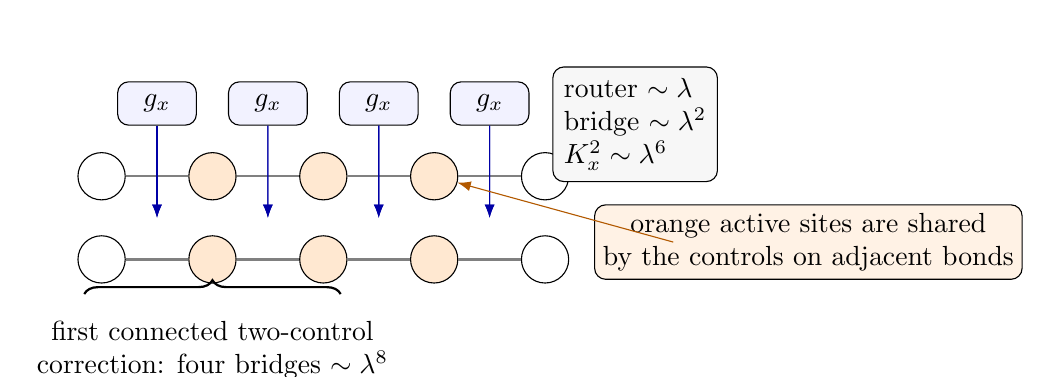
\begin{tikzpicture}[>=Latex,scale=0.88]
 \foreach \x in {0,4} {
   \node[circle,draw,minimum size=6mm] (u\x) at (1.6*\x,0.6) {};
   \node[circle,draw,minimum size=6mm] (d\x) at (1.6*\x,-0.6) {};
 }
 \foreach \x in {1,2,3} {
   \node[circle,draw,fill=orange!18,minimum size=6mm] (u\x) at (1.6*\x,0.6) {};
   \node[circle,draw,fill=orange!18,minimum size=6mm] (d\x) at (1.6*\x,-0.6) {};
 }
 \foreach \x in {0,1,2,3} {
   \pgfmathtruncatemacro{\y}{\x+1}
   \draw[gray,thick] (u\x) -- (u\y);
   \draw[gray,thick] (d\x) -- (d\y);
   \node[rectangle,draw,rounded corners,fill=blue!5,minimum width=1.0cm,minimum height=0.55cm] (g\x) at (0.8+1.6*\x,1.65) {$g_x$};
   \draw[->,blue!65!black] (g\x) -- ($(u\x)!0.5!(d\y)$);
   \draw[->,blue!65!black] (g\x) -- ($(d\x)!0.5!(u\y)$);
 }
 \draw[decorate,decoration={brace,amplitude=5pt},thick] (-0.25,-1.1) -- (3.45,-1.1)
 node[midway,below=6pt,align=center] {first connected two-control\\correction: four bridges $\sim\lambda^8$};
 \node[draw,rounded corners,fill=gray!6,align=left,inner sep=4pt] at (7.7,1.35) {router $\sim\lambda$\\bridge $\sim\lambda^2$\\$K_x^2\sim\lambda^6$};
 \node[draw,rounded corners,fill=orange!10,align=center,inner sep=3pt] at (10.2,-0.35)
 {orange active sites are shared\\by the controls on adjacent bonds};
 \draw[->,orange!70!black] (8.25,-0.35) -- (u3);
\end{tikzpicture}
\caption{Periodic array of overlapping controls.  Orange active sites belong to both adjacent bond controls, so isolated-bond Schur complements do not add exactly.  Weighted selection rules nevertheless delay the first connected overlap correction to order $\lambda^8$.}
\label{fig:global-gadgets}
\end{figure}

\subsection{Weighted selection rules and matched coefficients}

Here the \emph{weighted degree} of a monomial is its total power of $\lambda$ after assigning weight one to a router, two to a bridge, four to the leading shell/screening terms, and six to the subleading shell/screening and base terms.  Appendix~\ref{app:weighted} relates this regrading explicitly to the ordinary analytic Schrieffer--Wolff series.

A bridge vertex toggles one control between $g$ and $m$, so a closed low-control virtual walk contains an even number of bridges.  The high control graph is bipartite, $m\leftrightarrow\{s,a\}$, so a walk beginning and ending in $m$ contains an even number of router vertices.  Therefore the only virtual structures below weighted degree eight are two bridges on one bond and two bridges plus two routers on one bond.  A connected process involving two distinct controls requires at least four bridges and begins at degree eight.

On active seniority zero, Lemma~\ref{lem:routing} gives
\begin{align}
 P_{\rm sz}B_xC_{s,x}^2B_xP_{\rm sz}&=4P_{\rm sz}(B_x^2-K_x^2)P_{\rm sz},\\
 P_{\rm sz}B_xC_{a,x}^2B_xP_{\rm sz}&=4P_{\rm sz}K_x^2P_{\rm sz}.
\end{align}
The virtual contribution through degree six is
\begin{equation}
\begin{aligned}
H_{\rm virt}^{[6]}={}&-\lambda^4\Delta\frac{b^2}{\bar\Delta_m}\sum_xB_x^2
-\lambda^6\Delta\frac{4b^2s^2}{\bar\Delta_m^2\bar\Delta_s}\sum_xB_x^2\\
&+\lambda^6\Delta\,\bar\alpha\sum_xK_x^2,
\end{aligned}
\label{eq:virt-six}
\end{equation}
where
\begin{equation}
 \boxed{\bar\alpha=\frac{4b^2}{\bar\Delta_m^2}
 \left(\frac{s^2}{\bar\Delta_s}-\frac{a^2}{\bar\Delta_a}\right).}
 \label{eq:alpha-bar}
\end{equation}
Choose
\begin{equation}
 \boxed{\beta_4=\frac{b^2}{\bar\Delta_m},
 \qquad
 \beta_6=\frac{4b^2s^2}{\bar\Delta_m^2\bar\Delta_s}.}
 \label{eq:betas}
\end{equation}
Positive $U_q,V_q$ realizing these $\beta_q$ always exist, for example by choosing any $U_q>4\beta_q$ and setting $V_q=U_q-4\beta_q$.  The $B_x^2$ terms then cancel through weighted degree six, while the linked charge polynomials remain unless \eqref{eq:Hscreen} is included.

\subsection{Mismatch tolerances and the generic unscreened regime}
\label{sec:tuning}

The exact screened family is a matched parameter submanifold, so its experimental cost should be stated quantitatively.  Write the realized shell coefficients and density counterchannel as
\begin{equation}
 \beta_q^{\rm phys}=\beta_q+\delta\beta_q,
 \qquad
 H_{\rm scr,L}^{\rm phys}=H_{\rm scr,L}
 +\Delta\bigl(\lambda^4\delta\cC_{4,L}+\lambda^6\delta\cC_{6,L}\bigr).
\end{equation}
Through weighted degree six the residual low-block interaction is
\begin{equation}
 \lambda^4\Delta\,\cE_{4,L}
 +\lambda^6\Delta\left[H_{\rm base,L}+\bar\alpha\sum_xK_x^2+\cE_{6,L}\right],
 \qquad
 \cE_{q,L}=\delta\beta_q\sum_xB_x^2+\delta\cC_{q,L}.
 \label{eq:mismatch-effective}
\end{equation}
A sufficient local-norm tolerance for the multiplicative term to remain the leading composition-scale interaction, with fractional design error $O(\varepsilon)+O(\lambda^2)$, is
\begin{equation}
 \boxed{
 \norm{\cE_{4}}_\mu\le \varepsilon\lambda^2\bar\alpha,
 \qquad
 \norm{\cE_{6}}_\mu\le \varepsilon\bar\alpha.}
 \label{eq:tuning-tolerance}
\end{equation}
Because $\norm{B_x^2}=16$ and all local shell operators have fixed norm, this implies the scalar scaling rules
\begin{equation}
 \delta\beta_4=O(\varepsilon\lambda^2\bar\alpha),
 \qquad
 \delta\beta_6=O(\varepsilon\bar\alpha).
 \label{eq:beta-tolerances}
\end{equation}
At fixed total pair number, a residual order-four monopole coefficient $\delta A_4$ produces
\begin{equation}
 \delta V_4^{(L)}(n_1,n_2)
 =16\delta A_4\frac{L-2}{L(L-1)}n_1n_2,
\end{equation}
whose energy density is $O(\delta A_4)$ at extensive filling.  Hence preserving order-six composition degeneracy likewise requires $\delta A_4=O(\varepsilon\lambda^2\bar\alpha)$; the order-six charge mismatch may be $O(\varepsilon\bar\alpha)$.  The $U_qN_x$ part is composition independent at fixed total filling and does not enter this particular degeneracy tolerance.

For a family whose microscopic coefficients are held independent of $\lambda$, exact asymptotic composition degeneracy therefore requires the order-four residuals to vanish.  At any fixed design value of $\lambda$, however, \eqref{eq:tuning-tolerance} defines a nonzero tolerance tube around the matched point.  The unscreened corollary is the generic alternative: it requires no cancellation and retains the complete physical order-four charge operator explicitly; its compression contains the selector, while its centered action controls leakage.

\subsection{Finite-order local Schrieffer--Wolff definition}

We use a local interaction norm $\norm{\Phi}_\mu$ with exponential support weight $\e^{\mu\operatorname{diam}X}$.  In one dimension the present even fermion Hamiltonian may be treated in the graded tensor product, or Jordan--Wigner transformed within each fixed total-parity sector, without changing support connectivity.

To connect the weighted hierarchy directly to the ordinary construction of Ref.~\cite{Bravyi2011}, introduce independent analytic variables
\begin{equation}
 H(\mathbf z)=H_0+z_1V_1+z_2V_2+z_4V_4+z_6V_6
\end{equation}
and only afterward restrict to $z_w=\lambda^w$.  Every coefficient generated by the Schrieffer--Wolff recursion is a finite multilinear sum of vertices, commutators, block projections, and the fixed inverse control Liouvillian.  Substitution therefore turns its multivariate Taylor series into an ordinary analytic series in $\lambda$, and the coefficient of $\lambda^r$ is exactly the sum of monomials whose vertex weights add to $r$.  Moreover,
\begin{equation}
 \norm{H(\lambda)-H_0}_\mu
 \le C_1|\lambda|+C_2|\lambda|^2+C_4|\lambda|^4+C_6|\lambda|^6
 \le C|\lambda|
\end{equation}
for small $\lambda$, so the same convergence radius and locality estimates apply after restriction.  Appendix~\ref{app:weighted} gives the support and overlap bookkeeping in detail.

For $\rho\in\{{\rm scr},{\rm uns}\}$, let $S_{L,\rho}^{[7]}(\lambda)$ be the anti-Hermitian local Schrieffer--Wolff generator for $\mathbb H_L^\rho$ truncated after weighted degree seven, and define
\begin{equation}
 U_{L,\rho}^{[7]}(\lambda)=\exp S_{L,\rho}^{[7]}(\lambda),
 \qquad
 \widetilde H_{L,\rho}^{[7]}=U_{L,\rho}^{[7]}\mathbb H_L^\rho U_{L,\rho}^{[7]\dagger},
 \qquad
 H_{\rm eff,L,\rho}^{[7]}=P_g\widetilde H_{L,\rho}^{[7]}P_g.
 \label{eq:Heff-definition}
\end{equation}
The statements below concern these explicitly defined low blocks and separately control the residual $P_g$--$Q_g$ couplings.

\begin{theorem}[Screened global multiplicative downfolding]
\label{thm:global-screened}
Assume finite local dimension, fixed finite interaction range, positive control gaps, uniformly bounded microscopic couplings, the matching \eqref{eq:betas}, the screening counterchannel \eqref{eq:Hscreen}, and
\begin{equation}
 \frac{s^2}{\bar\Delta_s}>\frac{a^2}{\bar\Delta_a}.
 \label{eq:positive-condition}
\end{equation}
Then there exist $\lambda_0,C_\mu,C_\mu',C>0$, independent of $L$, such that for $\abs\lambda<\lambda_0$,
\begin{equation}
\boxed{
P_{\rm sz}H_{\rm eff,L,{\rm scr}}^{[7]}P_{\rm sz}
=\lambda^6\Delta P_{\rm sz}\left[H_{\rm base,L}+\bar\alpha\sum_xK_x^\dagger K_x\right]P_{\rm sz}+R_L^{(8)}.
}
\label{eq:global-screened-theorem}
\end{equation}
The low-block remainder and residual block coupling are generated by translation-invariant quasi-local interactions satisfying
\begin{align}
 \norm{\mathcal R_L^{(8)}}_\mu&\le C_\mu\Delta\abs\lambda^8,
 &\norm{R_L^{(8)}}&\le CL\Delta\abs\lambda^8,
 \label{eq:remainder-screened}\\
 \norm{Q_g\widetilde H_{L,{\rm scr}}^{[7]}P_g}_\mu&\le C_\mu'\Delta\abs\lambda^8.
 \label{eq:offdiag-screened}
\end{align}
The low-energy spectral and ground-energy errors are bounded by the same extensive order.
\end{theorem}

\begin{proof}
The unperturbed low subspace is a tensor product of local control ground states with the complete active Hilbert space.  The perturbation is analytic, finite range, and bounded in local norm.  The local Schrieffer--Wolff recursion therefore produces a finite-order anti-Hermitian generator, a linked-cluster low block, and a residual off-diagonal interaction whose first omitted coefficient has weighted degree eight \cite{Bravyi2011}.

The control selection rules enumerate every closed low-control walk below degree eight.  Only the one-bond coefficients in \eqref{eq:virt-six} survive.  A cluster containing two distinct control labels needs two bridge toggles for each label and hence begins with four bridges at weighted degree eight.  Shell, screening, and base vertices can extend the active support of a connected cluster, but they are diagonal in every control occupation and cannot replace any of those toggles; since their smallest weight is four, inserting one beside a one-control two-bridge process also begins at degree eight.  The detailed regraded linked-cluster argument is recorded in Appendix~\ref{app:weighted}.

The shell choices \eqref{eq:betas} cancel the ordinary $B_x^2$ terms, and \eqref{eq:Hscreen} cancels the linked monopole polynomials through degree six.  The surviving degree-six active interaction is therefore the displayed base parent plus the positive coefficient \eqref{eq:alpha-bar}.  Standard local truncation and cluster counting give the volume-independent interaction-norm bounds and the extensive operator-norm estimate.
\end{proof}

\begin{corollary}[Unscreened charge-selection family]
\label{cor:global-unscreened}
Under the hypotheses of \cref{thm:global-screened} except for \eqref{eq:Hscreen}, the same finite-order unitary satisfies
\begin{equation}
\boxed{
\begin{aligned}
P_{\rm sz}H_{\rm eff,L,{\rm uns}}^{[7]}P_{\rm sz}
={}&\lambda^4\Delta P_{\rm sz}\cC_{4,L}P_{\rm sz}\\
&+\lambda^6\Delta P_{\rm sz}\left[H_{\rm base,L}+\cC_{6,L}+\bar\alpha\sum_xK_x^\dagger K_x\right]P_{\rm sz}
+R_{L,{\rm uns}}^{(8)},
\end{aligned}}
\label{eq:global-unscreened-theorem}
\end{equation}
with the same local, global, and residual block-coupling orders.  At fixed total pair number $n$, the order-$\lambda^4$ projection onto the product-AGP composition basis contains
\begin{equation}
 \lambda^4\Delta\left[C_{4,L}(n)+16A_4\frac{L-2}{L(L-1)}n_1n_2\right].
 \label{eq:unscreened-selector}
\end{equation}
Thus the compression to the product-AGP composition space contains an order-$\lambda^4$ diagonal selector.  Proposition~\ref{prop:charge-leakage-periodic} shows that the same charge operator generally has order-$\lambda^4$ off-manifold singular values.  Without an additional order-four isolation mechanism, \eqref{eq:unscreened-selector} is therefore a projected selector law rather than the spectrum of an autonomous low-energy composition multiplet.
\end{corollary}

\begin{remark}[What is and is not exact]
The exact global Feshbach map is not a sum of isolated-bond Schur complements, because neighboring controls share active sites.  The theorem instead states that overlap cannot renormalize the order-six multiplicative coefficient: all connected overlap terms begin at order eight.  The effective order-six energy density has relative error $O(\lambda^2)$ in the screened family.  In the unscreened family the leading active operator is the complete order-four charge-selection term; its compression contains the selector \eqref{eq:unscreened-selector}, while Proposition~\ref{prop:charge-leakage-periodic} quantifies the accompanying off-manifold coupling.
\end{remark}

\subsection{Complete Peierls covariance and derivative control}

Use covering-lattice coordinates
\begin{equation}
 R(c_{a,x,\sigma})=x,
 \qquad
 R(r_{x,g})=R(r_{x,m})=R(r_{x,s})=R(r_{x,a})=x+\tfrac12.
 \label{eq:position-assignment}
\end{equation}
All control orbitals are co-located at the bond center; their internal transitions have zero displacement.  The elementary active--control monomials then have the displacements shown in \cref{tab:displacements}.

\begin{table}[H]
\centering
\caption{Covering-lattice displacement of representative factorized microscopic vertices.  Hermitian conjugation reverses the sign.}
\label{tab:displacements}
\begin{tabular}{@{}llc@{}}
\toprule
Vertex & Representative factorized vertex & $\Delta R$\\
\midrule
Bridge & $c_{1,x+1,\sigma}^\dagger c_{2,x,\sigma}E^x_{mg}$ & $+1$\\
Bridge & $c_{1,x,\sigma}^\dagger c_{2,x+1,\sigma}E^x_{mg}$ & $-1$\\
Same-chirality router & $c_{a,x+1,\sigma}^\dagger c_{a,x,\sigma}E^x_{sm}$ & $+1$\\
Opposite-chirality router & $c_{a,x,\sigma}^\dagger c_{a,x+1,\sigma}E^x_{am}$ & $-1$\\
Control energies/shell densities & $E^x_{\mu\mu}$, $N_x$, $N_x^2$ & $0$\\
\bottomrule
\end{tabular}
\end{table}

Twist each microscopic normal-ordered monomial by
\begin{equation}
 \mathcal O(A)=\e^{-\I A\Delta R(\mathcal O)}\mathcal O(0).
 \label{eq:peierls-monomial}
\end{equation}
On the boundary bond the unreduced covering coordinate is retained, so $A$ threads total flux $LA$.  No bridge, current, exchange kernel, or factor inside a composite vertex is held fixed while another is twisted.

\begin{corollary}[Peierls-covariant downfolding with derivative bounds]
\label{cor:peierls}
For either microscopic family, the conclusions of Theorem~\ref{thm:global-screened} and Corollary~\ref{cor:global-unscreened} hold uniformly for complex $A$ in a fixed strip $\abs{\operatorname{Im}A}<A_0$.  In particular, for every $0\le r\le2$ and every $0<\mu'<\mu$,
\begin{equation}
 \boxed{\norm{\partial_A^r\mathcal R_L^{(8)}(A)}_{\mu'}
 \le C_{\mu',r}\Delta\abs\lambda^8,}
 \qquad
 \boxed{\norm{\partial_A^rR_L^{(8)}(A)}
 \le C_rL\Delta\abs\lambda^8.}
 \label{eq:peierls-derivative-bound}
\end{equation}
The same derivative order holds for the residual $P_g$--$Q_g$ coupling.
\end{corollary}

\begin{proof}
The Peierls action is multiplicative in displacement and is respected by sums, products, commutators, the $P_g/Q_g$ projections, and inversion of the twist-independent control Liouvillian.  Hence every coefficient in the finite-order Schrieffer--Wolff recursion transforms covariantly.  The local interaction is analytic in a complex strip because every microscopic displacement is bounded.  The uniform strip bound, followed by a Cauchy estimate and a small reduction from $\mu$ to $\mu'$, gives \eqref{eq:peierls-derivative-bound}.
\end{proof}

\subsection{Explicit one-pair composition curvature}

Let $P_{\cZ_1}$ project onto the one-pair product-AGP basis $(\ket{1,0},\ket{0,1})$, and use the physical twist convention of \eqref{eq:peierls-monomial}.  In the screened family, the directional composition-curvature matrix is
\begin{equation}
\boxed{
 Q_{\rm comp}^{(1)}
 =2\lambda^6\Delta
 \begin{pmatrix}j_1&0\\0&j_2\end{pmatrix}
 +8\lambda^6\Delta\bar\alpha
 \begin{pmatrix}1&-1\\-1&1\end{pmatrix}
 +O(\Delta\lambda^8).
}
\label{eq:one-pair-curvature}
\end{equation}
The $O(\lambda^8)$ statement includes the first two twist derivatives by Corollary~\ref{cor:peierls}.  The off-diagonal entry is therefore nonzero whenever $\bar\alpha>0$.  In the one-pair periodic sector, Proposition~\ref{prop:charge-leakage-periodic} gives zero order-four leakage and \eqref{eq:unscreened-selector} vanishes, so the unscreened charge term does not alter \eqref{eq:one-pair-curvature}.  At higher fillings the complete order-four charge-selection operator must be resolved before the order-six composition curvature is interpreted.

\section{Numerical certificates and reproducibility}
\label{sec:numerics}

All computations use exact fermionic signs in fixed occupation bases.  The reported floating-point runs are machine-precision finite-Fock-space certificates of exact analytic identities; they are not substitutes for the proofs.  The principal checks are summarized in \cref{tab:certificates}.

\begin{table}[H]
\centering
\caption{Selected independent checks from the supplied certificates.  The global rows are restricted to the one-pair active sector.}
\label{tab:certificates}
\begin{tabular}{@{}p{0.52\linewidth}r@{}}
\toprule
Check & Error or result\\
\midrule
$[Q_a,B]$, full-Fock normal ordering, seniority-zero reduction & $0$\\
Sharp bound $\min\spec(9Q_a-K^2)$ & $-6.50\times10^{-15}$\\
Rank-three spectrum of $K^2|_{\rm sz}$ & $\{0^{\times13},4^{\times3}\}$\\
Compensated local Schur complement & $4.63\times10^{-15}$\\
Twisted local Schur complement & $4.66\times10^{-15}$\\
Plaquette analytic/Feshbach fourth-order coefficient & $6.94\times10^{-18}$\\
Plaquette analytic limit for $(E_a-E_s)/t^4$ & $0.044812246105$\\
Plaquette $t=0.02$: $(E_a-E_s)/t^4$ & $0.044811672577$\\
All-filling current-routing identities & $\le1.84\times10^{-15}$\\
Full-Fock minimum eigenvalue of $D$ & $8$\\
All-filling nested Schur complement & $2.23\times10^{-17}$\\
Kramers microscopic time-reversal residuals & $0$\\
Kramers closed-shell effective error divided by $\lambda^8$ & $\to2.42\times10^{-3}$\\
Product-AGP charge projection, all tests through $L=6$ & $5.68\times10^{-14}$\\
Exact periodic/open leakage formulas and zero sets, $L=2,\ldots,9$ & $15/15$ PASS\\
$L=4$, $(n_1,n_2)=(2,0)$ leakage norm divided by $A_4$ & $8\sqrt2/3$\\
One-pair, three-cell translation commutator & $2.22\times10^{-16}$\\
One-pair, two-cell effective error divided by $\lambda^8$ & $\to7.63\times10^{-3}$\\
\bottomrule
\end{tabular}
\end{table}

The local multiplet certificate also verifies the passive positivity window, unchanged kernel dimension, and one-pair composition curvature.  The electron-only certificate diagonalizes the full four-site plaquette and confirms convergence to \eqref{eq:Jparity}.  The all-filling certificate evaluates the exact source-range algebra on the full four-orbital Fock space, checks the charge formula by direct AGP enumeration, and confirms the $t_B^4$ feedback law.

A separate exact-arithmetic leakage verifier checks \cref{prop:charge-leakage-periodic,cor:charge-leakage-open} for both boundaries and every composition through $L=9$, totaling 760 boundary/composition sectors and 699,040 hard-core configuration evaluations.  Its centered-action checks establish zero mean and the exact variance in every composition.  The operator-level SVD then follows analytically from diagonality in the occupation basis together with orthogonality of distinct block-charge sectors; no floating-point Fock-space SVD is used.

The global certificate is deliberately narrower.  It uses active particle number two: the overlapping Feshbach test is performed on $L=3$, and the canonical low-energy extraction on $L=2$.  It therefore audits translation invariance, evenness in the bridge, the first overlap power, and the $\lambda^8$ one-pair scaling.  The all-filling and volume-uniform conclusions are analytic consequences of \cref{thm:global-screened}, not numerically certified by that script.  Moreover, because the selector coefficient in \eqref{eq:charge-selector} and the periodic leakage both vanish at $L=2$, the weighted two-cell extraction cannot diagnose either component of the leading unscreened monopole effect.

The complete repository certificate suite records the Python, NumPy, and SciPy versions in \texttt{ENVIRONMENT.txt}, lists SHA-256 hashes in \texttt{SHA256SUMS}, and contains six verifier programs and their raw certificate outputs.  Because last-digit eigensolver residuals depend on the BLAS/LAPACK build, \texttt{PLATFORM\_STABLE\_CERTIFICATE\_SUMMARY.txt} reports thresholded PASS/FAIL statements and rounded invariant values for portable diffs.
\section{Discussion}
\label{sec:discussion}

\subsection{Microscopic interpretation}

The multiplicative row is a symmetry-conditioned correlated-hopping channel.  The transfer $B_x$ creates a broken-pair source from every seniority-zero local configuration.  Current paths in the two blocks then interfere according to simultaneous endpoint parity.  The control sector converts that interference into two effective denominators.  An allowed orbital-polarization Coulomb channel cancels the parity-independent $B_x^2$ part, while an independently specified density counterchannel is required if the linked monopole polynomial is also to be removed.

No microscopic vertex contains $Q_a$ or $K$.  The parity projector appears only after ordinary electron paths are reduced.  The plaquette independently demonstrates that the required parity ordering can be generated by one-electron hopping, an onsite seniority gap, and density repulsion at fourth order, consistent with the broader appearance of cyclic and multiparticle exchange in strong-coupling expansions \cite{MacDonald1988,Aligia2018}.

\subsection{Relation to perturbative gadgets}

The control cluster belongs structurally to the mediator-gadget tradition: virtual ancillary levels simulate a target interaction that is not present as a primitive vertex \cite{Kempe2006,Oliveira2008,Jordan2008}.  Standard gadget analyses focus on approximate low-energy Hamiltonian simulation and on controlling cross-gadget errors.  Here the genuinely new ingredient is earlier in the construction: Lemma~\ref{lem:routing} is an exact full-source identity, independent of filling and of the control gaps.  The subsequent Schur complement and weighted overlap theorem then convert that exact router into the desired coefficient.  This separation between an exact algebraic router and perturbative energetic elimination is why the target survives on the complete seniority-zero space rather than only in a chosen code sector.

\subsection{Relation to the one-body obstruction}

Appendix~\ref{app:no-go} proves, within this paper, that exact additive one-body null rows under a complete local Peierls lift have composition-diagonal curvature.  The present mechanism crosses that boundary in the minimal structural way: all assumptions of that theorem are retained except additive one-body row structure.  This is minimality in hypothesis space, not a proof of minimal orbital number, interaction degree, or gadget complexity.  The unpublished companion manuscript \cite{SledgianowskiNoGo} contains the broader development but is not required to verify the logical step used here.

\subsection{Screened parent and physical selector}

The screened theorem and unscreened corollary describe distinct physical questions.  With explicit monopole screening and the matching tolerances \eqref{eq:tuning-tolerance}, the leading low-energy active Hamiltonian is the approximately composition-degenerate QGN parent
\begin{equation}
 H_{\rm base}+\bar\alpha\sum_xK_x^2
\end{equation}
with fractional design error $O(\varepsilon)+O(\lambda^2)$.  Exact asymptotic degeneracy is a tuned submanifold, whereas a finite experimental or numerical design has the nonzero tolerance tube quantified in \cref{sec:tuning}.  Without screening, the actual repulsive molecular shell generically produces a complete order-four charge-selection operator whose product-AGP compression is \eqref{eq:unscreened-selector}, followed by the order-six multiplicative channel.  The generic unscreened family is therefore a robust charge-selection problem.  As \cref{rem:order-four-isolation-gate} makes explicit, it becomes an autonomous selector-plus-mixing composition model only after an additional mechanism isolates the product-AGP manifold at order four or stronger.
In the two-sided row-ideal terminology developed for microscopic response transfer, $R_{{\rm ch},L}^{(n)}=(1-P_{\mathcal Z_n})H_{\rm ch}P_{\mathcal Z_n}$ is precisely the leading unscreened state source: an exact compression $P_{\mathcal Z_n}H_{\rm ch}P_{\mathcal Z_n}$ does not imply invariance of $\mathcal Z_n$ \cite{SledgianowskiMeissnerTransfer}.

\subsection{Limitations and remaining work}

The construction uses a general multiorbital two-electron interaction tensor.  The normal-ordered vertices \eqref{eq:normal-four-fermion} are allowed exchange or correlated-hopping matrix elements in ligand, layer, molecular-orbital, and moire Wannier descriptions, but their size has not been extracted from a specific material.  In particular, no general symmetry is claimed to enforce the same-chirality dominance $s^2/\bar\Delta_s>a^2/\bar\Delta_a$; it is an open parameter inequality whose sign must be established microscopically.  A derivation using only onsite density-density Hubbard $U$ would require another higher-order downfolding and is not claimed here.

The global theorem is perturbative and local.  It controls a finite-order approximately block-diagonal Hamiltonian, not an exact finite-coupling sum of isolated gadgets.  The first overlap corrections are bounded by order and support but are not classified term by term.  The base two-block QGN parent is an input, so the result supplies a controlled multiorbital UV construction of the additional multiplicative escape channel rather than a complete one-body projected-Hubbard realization.

Finally, the Peierls-covariant effective Hamiltonian controls static flux curvature.  Identifying that curvature with a dynamical zero-frequency Meissner or superfluid response requires additional gap and order-of-limits arguments and is not claimed here.

\section{Conclusion}

Multiplicative QGN null interactions need not be treated as formal positive-square gadgets.  Their local operator content is conventional, their parity selector can emerge from Pauli interference and correlated plaquette motion, and their compensating $B^2$ channel is realized by an explicit repulsive multiorbital constant-interaction tensor.  The all-filling identities
\begin{equation}
 C_s^2BP_0=4Q_sBP_0,
 \qquad
 C_a^2BP_0=4Q_aBP_0
\end{equation}
provide the exact bridge between microscopic paths and the emergent parity projector.  Under the full high-block gap $D\succeq d_*\Id>0$, the nested control sector produces the complete local $K^\dagger K$ channel at every product-AGP filling.

On a periodic lattice, a weighted hierarchy places that channel at order $\lambda^6$ and delays connected overlap, Kramers double-excitation, and residual block-coupling errors to order $\lambda^8$.  The screened family yields a composition-degenerate, translation-invariant, Peierls-covariant effective parent only on the matched submanifold, with the finite-$\lambda$ tolerance quantified in \eqref{eq:tuning-tolerance}.  The generic unscreened family retains the physically linked order-$\lambda^4$ charge-selection operator.  Its exact product-AGP compression contains the advertised diagonal selector, while its explicit singular values show that an isolated selector-plus-mixing composition model requires additional order-four protection.  The result completes a controlled multiorbital UV construction of the additional multiplicative escape channel, conditional on the base two-block QGN parent.  Material extraction and dynamical transport remain separate stages.


\appendix

\section{Self-contained additive one-body Peierls obstruction}
\label{app:no-go}

This appendix records the precise theorem whose boundary motivates the multiplicative row, so the present manuscript can be evaluated without access to the companion papers.  Let the paired one-particle space decompose into isolated interaction blocks
\begin{equation}
 \mathfrak h=\bigoplus_{a=1}^q\mathfrak h_a,
\end{equation}
with separate one-pair AGPs $\ket{\mathbf e_a}$ and fixed-total-pair product-AGP space $\cZ_n$.  Consider an analytic positive-square family
\begin{equation}
 H(A)=\frac12\sum_\ell S_\ell(A)^\dagger S_\ell(A)
      =\frac12\mathcal D(A)^\dagger\mathcal D(A),
 \qquad
 \mathcal D(A)\ket\psi=(S_\ell(A)\ket\psi)_\ell.
 \label{eq:nogo-positive}
\end{equation}
Assume $\ker\mathcal D(0)=\cZ_n$ in the sector considered.  For a twist direction $v$, define the stacked source and its frustration-free projection by
\begin{equation}
 \mathcal B_v\ket\psi=(\partial_vS_\ell(0)\ket\psi)_\ell,
 \qquad
 T_v=P_{\ker\mathcal D(0)^\dagger}\mathcal B_v\big|_{\cZ_n},
 \qquad
 Q_v^{(n)}=T_v^\dagger T_v.
 \label{eq:nogo-curvature}
\end{equation}
The matrix $Q_v^{(n)}$ is the exact second-order frustration-free curvature operator on the zero manifold.

\begin{lemma}[One-pair rigidity]
\label{lem:nogo-rigidity}
Let $S=\mathrm d\Gamma(s)$ be a number-conserving one-body row and suppose $S\ket{\mathbf e_b}=0$ for every separate one-pair state.  Then every interblock matrix block vanishes:
\begin{equation}
 P_asP_b=0\qquad(a\ne b).
\end{equation}
\end{lemma}

\begin{proof}
Fix $a\ne b$, put $x=P_asP_b$, and project $S\ket{\mathbf e_b}$ onto the charge sector with one fermion in block $a$ and one in block $b$.  The projected component is $c_a^\dagger x c_b\ket{\mathbf e_b}$.  The target block is empty and the one-body density matrix of the normalized one-pair AGP in block $b$ is $\mathbb I_{2L_b}/L_b$, hence
\begin{equation}
 \norm{c_a^\dagger x c_b\ket{\mathbf e_b}}^2
 =\frac1{L_b}\Tr(x^\dagger x).
\end{equation}
The left side vanishes, so $x=0$.
\end{proof}

\begin{theorem}[Peierls-transport obstruction]
\label{thm:self-contained-nogo}
Assume:
\begin{enumerate}[label=\textup{(H\arabic*)},leftmargin=3.8em]
 \item $H(A)$ has the analytic positive-square form \eqref{eq:nogo-positive};
 \item every $S_\ell(A)$ is a number-conserving one-body row;
 \item the same zero-twist factor family annihilates every $\ket{\mathbf e_a}$ and has complete fixed-$n$ kernel $\cZ_n$;
 \item the interaction singular subbundles are isolated and analytic; and
 \item the physical field dependence is the complete covering-lattice Peierls shift of fixed finite-range or uniformly exponentially local kernels.
\end{enumerate}
Then the exact curvature map preserves every block composition:
\begin{equation}
 \boxed{(Q_v^{(n)})_{\mathbf m\mathbf n}=0\qquad(\mathbf m\ne\mathbf n).}
 \label{eq:nogo-conclusion}
\end{equation}
A physical twist may give distinct diagonal block masses and a nontrivial lower envelope, but no Jacobi hopping between exact one-body interaction blocks.
\end{theorem}

\begin{proof}
Lemma~\ref{lem:nogo-rigidity} makes every zero-twist row block preserving.  The complete Peierls shift preserves the corresponding shifted projectors $P_a(A)$.  Since these projectors form an isolated analytic orthogonal family, Kato transport supplies one analytic one-particle unitary $R(A)$, common to every row label, satisfying $R(A)P_aR(A)^\dagger=P_a(A)$ \cite[Chap.~II]{Kato1976}.  Let $\widehat R(A)$ be its number-conserving Fock lift and write
\begin{equation}
 S_\ell(A)=\widehat R(A)\widetilde S_\ell(A)\widehat R(A)^\dagger,
\end{equation}
where every $\widetilde S_\ell(A)$ preserves the fixed block charges.  Differentiation at $A=0$ gives
\begin{equation}
 \partial_vS_\ell(0)=[G_v,S_\ell(0)]+\widetilde B_{\ell v}^{\rm bp},
 \qquad
 G_v=\partial_v\widehat R(0),
\end{equation}
with $\widetilde B_{\ell v}^{\rm bp}$ block preserving.  For $\ket\psi\in\cZ_n$,
\begin{equation}
 [G_v,S_\ell]\ket\psi=-S_\ell G_v\ket\psi,
\end{equation}
so the stacked commutator source lies in $\operatorname{ran}\mathcal D(0)$ and is annihilated by $P_{\ker\mathcal D(0)^\dagger}$.  The surviving projected source preserves every block charge.  Sources from distinct compositions therefore occupy orthogonal charge sectors, which proves \eqref{eq:nogo-conclusion}.
\end{proof}

The row $K_x=Q_{a,x}B_x$ retains analyticity, number conservation, finite range, the complete product-AGP kernel, and termwise Peierls covariance, but violates hypothesis (H2): it is multiplicative and many body rather than additive and one body.  This is the precise sense in which it is the minimal structural escape.

\section{Base-kernel details}
\label{app:base-kernel}

In seniority zero, identify an occupied onsite pair with a hard-core bit.  For fixed $n_a$, a basis state in block $a$ is labeled by an $n_a$-element subset $S\subset\Lambda_L$.  The adjacent swaps generate the natural transitive action of $S_L$ on such subsets.  A vector fixed by every adjacent swap must assign the same coefficient to every $S$, and hence is proportional to
\begin{equation}
 \binom{L}{n_a}^{-1/2}\sum_{|S|=n_a}\prod_{x\in S}d_{a,x}^\dagger\ket0.
\end{equation}
This is precisely the normalized block AGP.  Tensoring the two blocks gives Proposition~\ref{prop:base-kernel}.


\section{One-block current table}
\label{app:current-table}

Use the mode order $(L\uparrow,L\downarrow,R\uparrow,R\downarrow)$.  In the one-electron basis $(\ket{L\sigma},\ket{R\sigma})$ and the one-hole basis $(\ket{D_L,R\sigma},\ket{L\sigma,D_R})$, the current and endpoint swap are
\begin{equation}
 J\big|_{N=1}=\begin{pmatrix}0&\I\\-\I&0\end{pmatrix},
 \qquad
 J\big|_{N=3}=\begin{pmatrix}0&-\I\\\I&0\end{pmatrix},
 \qquad
 W=\begin{pmatrix}0&1\\1&0\end{pmatrix}.
 \label{eq:odd-current-matrices}
\end{equation}
Thus $J^2=1$ in both odd sectors.  On the seniority-zero two-particle basis $(\ket{D_L},\ket{D_R})$,
\begin{equation}
 J^2=2\begin{pmatrix}1&-1\\-1&1\end{pmatrix}=2(1-W)=4\Pi,
 \label{eq:doublon-current-square}
\end{equation}
while $J$ vanishes on $\ket0$ and $\ket{D_LD_R}$.  These matrices prove the one-block statements in Lemma~\ref{lem:routing}.  To check the two-block source identity, apply the four crossed hopping directions to the $16$ seniority-zero occupation states.  The nonzero images fall into the four odd-sector classes $(N_1,N_2)=(1,1),(1,3),(3,1),(3,3)$.  In each class, the matrices in \eqref{eq:odd-current-matrices}, together with the graded fermionic sign from the global mode ordering and the crossed endpoint orientation, give $(J_1J_2-W_1W_2)B\ket z=0$.  This finite basis table proves \eqref{eq:range-current2} without invoking a numerical diagonalization.

\section{Kramers-doubled time-reversal embedding}
\label{app:kramers}

Let $\kappa=\pm$ label a Kramers pair for every control orbital and define $E_{\mu\nu}^{\kappa}=r_{\mu\kappa}^\dagger r_{\nu\kappa}$ and $\chi_+=1$, $\chi_-=-1$.  Choose phases such that
\begin{equation}
 \Theta r_{\mu,+}\Theta^{-1}=r_{\mu,-},
 \qquad
 \Theta r_{\mu,-}\Theta^{-1}=-r_{\mu,+},
 \qquad
 \Theta\I\Theta^{-1}=-\I.
 \label{eq:kramers-action}
\end{equation}
The active transfer is time-reversal even, $\Theta B\Theta^{-1}=B$, whereas the orbital currents are odd, $\Theta C_{s,a}\Theta^{-1}=-C_{s,a}$.  The doubled control Hamiltonian
\begin{equation}
\begin{aligned}
 H_{\rm ctrl}^{\Theta}=\sum_{\kappa=\pm}\bigl[&
 \Delta_mE_{mm}^{\kappa}+\Delta_s^{(r)}E_{ss}^{\kappa}+\Delta_a^{(r)}E_{aa}^{\kappa}
 +t_BB(E_{mg}^{\kappa}+E_{gm}^{\kappa})\\
 &+\chi_\kappa t_sC_s(E_{sm}^{\kappa}+E_{ms}^{\kappa})
 +\chi_\kappa t_aC_a(E_{am}^{\kappa}+E_{ma}^{\kappa})\bigr]
 \label{eq:kramers-H}
\end{aligned}
\end{equation}
is invariant under $\Theta$: the two control transitions are exchanged, while the signs of both $\chi_\kappa$ and the active current reverse.

With one control electron, the low $g$ level is a Kramers doublet.  The two $\kappa$ sectors do not mix, and their high operators are
\begin{equation}
 D_\kappa=\Delta_m-\frac{(\chi_\kappa t_s)^2}{\Delta_s^{(r)}}C_s^2
                    -\frac{(\chi_\kappa t_a)^2}{\Delta_a^{(r)}}C_a^2=D.
\end{equation}
Consequently the exact Schur complement is the operator in Theorem~\ref{thm:all-filling} tensored with the identity on the Kramers doublet.  This proves the reviewer's requested equality of partner coefficients, but it leaves a spectator Kramers degeneracy, as required for any odd-electron time-reversal-invariant control.

A unique local control ground state is obtained by replacing the one-electron charging term with $U_r(N_r-2)^2$ and fixing two control electrons in the closed shell
\begin{equation}
 \ket G=r_{g,+}^\dagger r_{g,-}^\dagger\ket0.
\end{equation}
Use the Hamiltonian \eqref{eq:kramers-H} with bridge amplitude $t_B/\sqrt2$ in each partner.  At weighted degree four, a virtual path excites and de-excites one of the two electrons; the two orthogonal choices contribute
\begin{equation}
 2\left(\frac{t_B}{\sqrt2}\right)^2=t_B^2.
\end{equation}
At degree six, both router insertions preserve the same Kramers label and $\chi_\kappa^2=1$, so the same factor reproduces the single-flavor $B^2$ and $K^2$ coefficients exactly.  A process that excites both Kramers electrons requires at least four bridge vertices and therefore begins at weighted degree eight.  Thus the closed-shell model is strictly time-reversal invariant, has a unique control ground state, and satisfies the screened and unscreened lattice theorems through degree six with only a change in the order-eight remainder constant.  The accompanying verifier performs an exact one-bond closed-shell Feshbach calculation and confirms the predicted $\lambda^8$ residual scaling.

\section{Plaquette path sum}
\label{app:plaquette}

Let $P=\ket A\bra A+\ket B\bra B$ and let $Q=1-P$ in the four-electron sector of \eqref{eq:plaquette}.  Write $H(t_p)=H_0+t_pT$.  Since $PTP=0$ and $c_{aR\sigma}\mapsto-c_{aR\sigma}$ sends $T\mapsto-T$, the effective doublet Hamiltonian contains only even powers.  Its second-order term is proportional to $P$, so the fourth-order folded contribution constructed from the second-order operator is also proportional to $P$ and does not affect the parity splitting.

The splitting is therefore determined by the connected off-diagonal path sum
\begin{equation}
 h_{AB}^{(4)}=-\bra A TQH_Q^{-1}QTQH_Q^{-1}QTQH_Q^{-1}QT\ket B.
\end{equation}
Grouping paths by whether the first broken-pair configuration has one or two occupied repulsive cycle edges yields denominators $V_p$, $2\Delta_p+V_p$, and $4\Delta_p+3V_p$.  Summing spin and ordering multiplicities gives
\begin{equation}
 h_{AB}^{(4)}=-\frac{128(2\Delta_p+3V_p)}{V_p(2\Delta_p+V_p)(4\Delta_p+3V_p)^2}t_p^4.
\end{equation}
The companion exact-diagonalization script constructs the full four-electron matrix and independently evaluates the same connected Feshbach coefficient.

\section{Charge combinatorics}
\label{app:charge}

Let $X_{a,x}\in\{0,1\}$ be the hard-core pair occupation in block $a$.  On $\ket{n_a}_a$,
\begin{equation}
 \langle X_{a,x}\rangle=\frac{n_a}{L},
 \qquad
 \langle X_{a,x}X_{a,y}\rangle=\frac{n_a(n_a-1)}{L(L-1)}
 \quad(x\ne y).
\end{equation}
The bond electron number is
\begin{equation}
 N_x=2(X_{1,x}+X_{1,x+1}+X_{2,x}+X_{2,x+1}).
\end{equation}
Expanding $N_x^2$, using translation invariance and factorization between blocks, and summing $x$ gives \eqref{eq:charge-potential}.  The absence of off-diagonal composition matrix elements in the compression follows because $N_x$ commutes with both block charges; the centered variance calculation in Proposition~\ref{prop:charge-leakage-periodic} determines the simultaneous off-manifold block.

\subsection{Open-path boundary formula for the numerical certificates}

\begin{corollary}[Open-path charge compression and leakage]
\label{cor:charge-leakage-open}
Consider the standard open truncation with $L$ active sites and bonds
$x=1,\ldots,L-1$.  Define
\[
 H_{{\rm ch},L}^{\rm op}
 =\sum_{x=1}^{L-1}\left(A_c N_x^2-\frac{U_c}{2}N_x\right),
 \qquad V_c=4A_c-U_c>0.
\]
Let
\[
 B_a=X_{a,1}+X_{a,L},\qquad
 E_a=\sum_{x=1}^{L-1}X_{a,x}X_{a,x+1},
\]
\[
 t_{a,x}=X_{a,x}+X_{a,x+1},\qquad
 C=\sum_{x=1}^{L-1}t_{1,x}t_{2,x},
 \qquad B=B_1+B_2,\quad Z=E_1+E_2+C.
\]
Then, configuration by configuration,
\begin{equation}
 \boxed{
 H_{{\rm ch},L}^{\rm op}
 =(8A_c-2U_c)n+8A_cZ-V_cB.}
 \label{eq:open-charge-decomposition}
\end{equation}
Its product-AGP compression is
\begin{equation}
 \boxed{
 \bra{n_1,n_2}H_{{\rm ch},L}^{\rm op}\ket{n_1,n_2}
 =C_L^{\rm op}(n)+16A_c\frac{L-2}{L^2}n_1n_2,}
 \label{eq:open-charge-selector}
\end{equation}
where
\begin{equation}
 C_L^{\rm op}(n)
 =\frac{8A_cn(L+n-2)-2U_cn(L-1)}{L}.
 \label{eq:open-charge-baseline}
\end{equation}
For $p_k(m)=(m)_k/(L)_k$, define
\begin{align}
 b_L(m)&=\frac{2m(L-m)(L-2)}{L^2(L-1)},
 &h_L(m)&=-\frac{2m(m-1)(L-m)}{L^2(L-1)},
 \label{eq:open-b-h}\\
 e_L(m)&=\frac{m(m-1)(L-m)(L-m+1)}{L^2(L-1)},
 \label{eq:open-e}
\end{align}
\[
 u_0(m)=2p_1(m)+2p_2(m),\qquad
 u_1(m)=p_1(m)+3p_2(m),\qquad
 u_2(m)=4p_2(m),
\]
\begin{align}
 w_L(n_1,n_2)={}&(L-1)u_0(n_1)u_0(n_2)
 +2(L-2)u_1(n_1)u_1(n_2)\notag\\
 &+(L-2)(L-3)u_2(n_1)u_2(n_2)
 -\left[\frac{4(L-1)n_1n_2}{L^2}\right]^2,
 \label{eq:open-w}
\end{align}
\begin{align}
 \Gamma_0={}&e_L(n_1)+e_L(n_2)+w_L(n_1,n_2)
 -\frac{4n_2}{L}h_L(n_1)-\frac{4n_1}{L}h_L(n_2),\notag\\
 \Gamma_1={}&h_L(n_1)+h_L(n_2)
 -\frac{2n_2}{L}b_L(n_1)-\frac{2n_1}{L}b_L(n_2),\notag\\
 \Gamma_2={}&b_L(n_1)+b_L(n_2).
 \label{eq:open-gammas}
\end{align}
For
\[
 R_{{\rm ch},L}^{(n),\rm op}
 =(1-P_{\mathcal Z_n})H_{{\rm ch},L}^{\rm op}P_{\mathcal Z_n},
\]
the singular value attached to composition $(n_1,n_2)$ is
\begin{equation}
 \boxed{
 (\tau_{L;n_1,n_2}^{\rm op})^2
 =64A_c^2\Gamma_0-16A_cV_c\Gamma_1+V_c^2\Gamma_2.}
 \label{eq:open-charge-leakage-variance}
\end{equation}
If $\tau_{L;c}^{\rm op}>0$, define
\[
 \ket{\ell_{L;c}^{\rm op}}
 =\frac{(H_{{\rm ch},L}^{\rm op}-\mu_{L;c}^{\rm op})\ket c}
 {\tau_{L;c}^{\rm op}}.
\]
Then
\begin{equation}
 \boxed{
 R_{{\rm ch},L}^{(n),\rm op}
 =\sum_{\substack{c=(n_1,n_2)\\n_1+n_2=n,\ \tau_{L;c}^{\rm op}>0}}
 \tau_{L;c}^{\rm op}\ket{\ell_{L;c}^{\rm op}}\bra c,
 \qquad
 \norm{R_{{\rm ch},L}^{(n),\rm op}}
 =\max_{n_1+n_2=n}\tau_{L;n_1,n_2}^{\rm op}.}
 \label{eq:open-charge-leakage-svd}
\end{equation}
For $L\ge3$, the open leakage vanishes exactly at
$(n_1,n_2)\in\{0,L\}\times\{0,L\}$.  For $L=2$, it vanishes in every sector.
\end{corollary}

\begin{proof}
The path identities
\[
 \sum_{x=1}^{L-1}N_x=4n-2B,
 \qquad
 \sum_{x=1}^{L-1}N_x^2=8n-4B+8Z
\]
prove \eqref{eq:open-charge-decomposition}.  Uniform fixed-size subset averages
give \eqref{eq:open-charge-selector}.

The quantities $b_L,h_L,e_L$ are respectively
$\operatorname{Var}(B_a)$, $\operatorname{Cov}(E_a,B_a)$, and
$\operatorname{Var}(E_a)$.  Counting equal, adjacent, and disjoint ordered edge
pairs proves $w_L=\operatorname{Var}(C)$.  Moreover
\[
 \mathbb E[C\mid X_1]=\frac{2n_2}{L}(2n_1-B_1),
\]
so
\[
 \operatorname{Cov}(C,E_1)=-\frac{2n_2}{L}h_L(n_1),
 \qquad
 \operatorname{Cov}(C,B_1)=-\frac{2n_2}{L}b_L(n_1),
\]
with the exchanged formulas for block $2$.  Hence
$\Gamma_0=\operatorname{Var}(Z)$,
$\Gamma_1=\operatorname{Cov}(Z,B)$, and
$\Gamma_2=\operatorname{Var}(B)$, proving
\eqref{eq:open-charge-leakage-variance} and the SVD.

Finally, $\Gamma_0\ge0$, $\Gamma_2\ge0$, and $\Gamma_1\le0$ because
$h_L(m)\le0$ and $b_L(m)\ge0$.  With $A_c,V_c>0$, every term in
\eqref{eq:open-charge-leakage-variance} is nonnegative.  Vanishing therefore
forces $\Gamma_2=0$, which for $L\ge3$ is equivalent to each block being empty
or full.  The converse is immediate.
\end{proof}

\begin{remark}[Boundary scope and shell normalization]
The global microscopic theorem is periodic, so
Proposition~\ref{prop:charge-leakage-periodic} is the theorem-level statement.
The open corollary is required when a numerical calculation removes the wrap
bond.  On the cycle,
\[
 \frac{\tau_{L;c}^{2,{\rm per}}}{A_c^2}=\sigma_L^2(c)
\]
is independent of $U_c$.  On the path,
\[
 \frac{(\tau_{L;c}^{\rm op})^2}{A_c^2}
 =64\Gamma_0-16\frac{V_c}{A_c}\Gamma_1
 +\left(\frac{V_c}{A_c}\right)^2\Gamma_2.
\]
Thus open normalization is exact under a common rescaling of the shell
parameters, but $V_c/A_c$ must be held fixed.  In the order-four microscopic
family, set $(A_c,U_c,V_c)=(A_4,U_4,V_4)$.
\end{remark}

\section{Weighted linked-cluster bookkeeping}
\label{app:weighted}

The ordinary local Schrieffer--Wolff construction is analytic in a perturbation $V$ and organizes every coefficient as a finite sum of nested commutators, block projections, inverse unperturbed Liouvillians, and local interaction vertices \cite{Bravyi2011}.  For the present hierarchy, introduce the multivariate family
\begin{equation}
 H(\mathbf z)=H_0+z_1V_1+z_2V_2+z_4V_4+z_6V_6.
 \label{eq:multivariate-SW}
\end{equation}
At any fixed ordinary recursion order, the generator and transformed Hamiltonian are multivariate polynomials in $(z_1,z_2,z_4,z_6)$.  Restricting to
\begin{equation}
 z_1=\lambda,
 \qquad z_2=\lambda^2,
 \qquad z_4=\lambda^4,
 \qquad z_6=\lambda^6
\end{equation}
therefore gives an analytic single-variable series whose $\lambda^r$ coefficient is exactly the sum of monomials with total vertex weight $r$.  This is a regrouping of the ordinary Taylor series, not a new formal expansion.

The locality and convergence estimates survive the restriction.  If the microscopic local norms are bounded by $M_w$, then
\begin{equation}
 \norm{H(\lambda)-H_0}_\mu
 \le M_1|\lambda|+M_2|\lambda|^2+M_4|\lambda|^4+M_6|\lambda|^6
 \le M|\lambda|
\end{equation}
for $|\lambda|\le1$.  Choosing $|\lambda|$ below the ordinary small-norm radius of the local Schrieffer--Wolff map yields the same exponential cluster bound.  Collecting all terms of weighted degree at most seven is therefore legitimate coefficient by coefficient, and the omitted interaction begins at weighted degree eight with constants independent of $L$.

It remains to justify the overlap threshold in the presence of control-diagonal vertices.  A control label can enter a virtual walk from the low state $g_x$ only through a bridge $g_x\leftrightarrow m_x$.  Every participating control must therefore be toggled by at least two bridges, one to leave $g_x$ and one to return.  A one-control closed walk begins with two bridges and has weight four.  Router vertices act only inside $m_x\leftrightarrow\{s_x,a_x\}$ and occur in pairs, so the target one-control path has weights $2+1+1+2=6$.

A connected contribution containing two distinct control labels requires at least two bridges for each label, hence at least four bridges and total weight eight.  Shell, screening, and base vertices are diagonal in all control occupations.  They may touch neighboring active sites and thereby enlarge the geometric support of a cluster, but they cannot cause a control to leave or re-enter $g_x$ and cannot reduce the required bridge count.  Their smallest weight is four, so a one-control two-bridge process decorated by any such adjacent vertex also begins at weight $4+4=8$.  The same argument applies to the closed-shell Kramers embedding: exciting both partners requires four bridges.  These observations prove that no connected overlap, control-diagonal support extension, or double-Kramers excitation can modify the degree-six single-control coefficient.

\section{Peierls covariance of the microscopic vertices}
\label{app:peierls}

For a normal-ordered monomial
\begin{equation}
 \mathcal O=C\,f_{x_1}^\dagger\cdots f_{x_p}^\dagger f_{y_p}\cdots f_{y_1},
\end{equation}
define the covering-lattice displacement
\begin{equation}
 \Delta R(\mathcal O)=\sum_{j=1}^px_j-\sum_{j=1}^py_j.
\end{equation}
The complete uniform twist is
\begin{equation}
 \mathcal O(A)=\e^{-\I A\Delta R(\mathcal O)}\mathcal O(0).
\end{equation}
The explicit embedding \eqref{eq:position-assignment} assigns zero displacement to every internal control transition and $\pm1$ to every active hop inside a bridge or router vertex.  Products and commutators add displacements, while $P_g$, $Q_g$, and the control Liouvillian have zero displacement.  Thus every finite-order Schrieffer--Wolff term carries exactly the phase of its effective normal-ordered monomial; the effective $K_x(A)^2$ is generated covariantly rather than by twisting only one factor of a composite operator.

For complex $A$, a local term supported on diameter $d$ acquires at most $\e^{\abs{\operatorname{Im}A}d}$.  Choosing $\abs{\operatorname{Im}A}<A_0<\mu-\mu'$ preserves the $\mu'$ interaction norm uniformly.  Cauchy's integral formula in this strip gives the derivative estimates in \eqref{eq:peierls-derivative-bound} for $r=1,2$.

\section{Certificate parameter sets}
\label{app:certificates}

The local multiplet audit uses $U_0=2$, $j_1=1$, $j_2=1.3$, $t=0.8$, $\Delta_s=12$, and $\Delta_a=20$.  The electron plaquette uses $\Delta_p=10$ and $V_p=3$.  The all-filling router uses $\Delta_m=10$, $\Delta_s^{(r)}=\Delta_a^{(r)}=8$, $t_s=1$, $t_a=1/2$, and $t_B=0.7$; for these values $\min\spec D=8$.  The direct-feedback sequence is included only to confirm the $t_B^4$ law, and the manuscript separately identifies the perturbative regime.

The Kramers closed-shell audit uses the same local gaps and currents, fixes two control electrons in $g_+g_-$, assigns bridge amplitude $b/\sqrt2$ to each partner, and verifies that the one-bond exact Feshbach map differs from the single-flavor degree-six target by $O(\lambda^8)$.

The global weighted audit uses active particle number two, $\bar\Delta_m=10$, $\bar\Delta_s=\bar\Delta_a=8$, $s=1$, $a=1/2$, and $b=0.7$, giving
\begin{equation}
 \bar\alpha=0.0018375.
\end{equation}
The exact canonical low-energy extraction on the two-cell periodic system gives
\begin{equation}
 \frac{\norm{H_{\rm eff}(\lambda)-\lambda^6\bar\alpha\sum_xK_x^2}}{\lambda^8}
 \longrightarrow 7.63\times10^{-3}
\end{equation}
in that one-pair sector.  The overlapping $L=3$ Feshbach audit is likewise one-pair only.  Neither computation is presented as an all-filling or volume-uniform numerical certificate.

\begin{thebibliography}{99}

\bibitem{Han2024}
Z. Han, J. Herzog-Arbeitman, B. A. Bernevig, and S. A. Kivelson,
``Quantum Geometric Nesting and Solvable Model Flat-Band Systems,''
\emph{Phys. Rev. X} \textbf{14}, 041004 (2024),
doi:10.1103/PhysRevX.14.041004.

\bibitem{Tovmasyan2016}
M. Tovmasyan, S. Peotta, P. T\"orm\"a, and S. D. Huber,
``Effective theory and emergent $SU(2)$ symmetry in the flat bands of attractive Hubbard models,''
\emph{Phys. Rev. B} \textbf{94}, 245149 (2016),
doi:10.1103/PhysRevB.94.245149.

\bibitem{Peotta2015}
S. Peotta and P. T\"orm\"a,
``Superfluidity in topologically nontrivial flat bands,''
\emph{Nat. Commun.} \textbf{6}, 8944 (2015),
doi:10.1038/ncomms9944.

\bibitem{Schrieffer1966}
J. R. Schrieffer and P. A. Wolff,
``Relation between the Anderson and Kondo Hamiltonians,''
\emph{Phys. Rev.} \textbf{149}, 491--492 (1966),
doi:10.1103/PhysRev.149.491.

\bibitem{MacDonald1988}
A. H. MacDonald, S. M. Girvin, and D. Yoshioka,
``$t/U$ expansion for the Hubbard model,''
\emph{Phys. Rev. B} \textbf{37}, 9753--9756 (1988),
doi:10.1103/PhysRevB.37.9753.

\bibitem{Kempe2006}
J. Kempe, A. Kitaev, and O. Regev,
``The complexity of the local Hamiltonian problem,''
\emph{SIAM J. Comput.} \textbf{35}, 1070--1097 (2006),
doi:10.1137/S0097539704445226.

\bibitem{Oliveira2008}
R. Oliveira and B. M. Terhal,
``The complexity of quantum spin systems on a two-dimensional square lattice,''
\emph{Quantum Inf. Comput.} \textbf{8}, 900--924 (2008),
arXiv:quant-ph/0504050.

\bibitem{Jordan2008}
S. P. Jordan and E. Farhi,
``Perturbative gadgets at arbitrary orders,''
\emph{Phys. Rev. A} \textbf{77}, 062329 (2008),
doi:10.1103/PhysRevA.77.062329.

\bibitem{Bravyi2011}
S. Bravyi, D. P. DiVincenzo, and D. Loss,
``Schrieffer--Wolff transformation for quantum many-body systems,''
\emph{Ann. Phys.} \textbf{326}, 2793--2826 (2011),
doi:10.1016/j.aop.2011.06.004.

\bibitem{Aligia2018}
A. A. Aligia,
``Calculation of the four-spin cyclic exchange in cuprates,''
\emph{Phys. Rev. B} \textbf{98}, 125118 (2018),
doi:10.1103/PhysRevB.98.125118.

\bibitem{Georges2013}
A. Georges, L. de' Medici, and J. Mravlje,
``Strong Correlations from Hund's Coupling,''
\emph{Annu. Rev. Condens. Matter Phys.} \textbf{4}, 137--178 (2013),
doi:10.1146/annurev-conmatphys-020911-125045.

\bibitem{Kato1976}
T. Kato,
\emph{Perturbation Theory for Linear Operators}, 2nd ed.
(Springer, Berlin, 1976).

\bibitem{SledgianowskiParent}
N. Sledgianowski,
``Exact Flat-Band Stiffness from Pair Mobility in a QGN Model: Finite-size obstructions, a many-body reduction theorem, and a proof of the Gao--Han--Khalaf formula for Model II,'' manuscript (2026).

\bibitem{SledgianowskiMultiBlock}
N. Sledgianowski,
``Multi-Block Reduction and Irreducibility Laws for QGN Superconductors,'' manuscript (2026).

\bibitem{SledgianowskiNoGo}
N. Sledgianowski,
``Peierls-Transport Obstruction and the Minimal Many-Body Escape,'' review-integrated manuscript (2026); the theorem used here is restated and proved in Appendix~\ref{app:no-go}.

\bibitem{SledgianowskiMeissnerTransfer}
N. Sledgianowski,
``Microscopic Transfer of Exact Meissner Weight,'' manuscript (2026).

\end{thebibliography}

\end{document}
